\documentclass[a4paper,12pt,titlepage]{article}
\usepackage[utf8]{inputenc}
\usepackage{a4wide}
\usepackage[czech]{babel}
\usepackage{amsfonts, amsmath, amsthm, amssymb}
\usepackage[small,compact]{titlesec}
\usepackage{anyfontsize}
\usepackage{rotating}
\usepackage{mdwlist}
\usepackage{xcolor}
\usepackage{graphicx}

\newcommand{\shn}{\Theta}
\newcommand{\lm}{\smallskip\noindent\bf Lemma\rm{} }
\newcommand{\dk}{\smallskip\noindent\bf Důkaz\rm{} }
\newcommand{\df}{\smallskip\noindent\bf Definice\rm{} }
\newcommand{\vt}{\smallskip\noindent\bf Věta\rm{} }
\newcommand{\pr}{\smallskip\noindent\bf Příklad\rm{} }
\newcommand{\poz}{\smallskip\noindent\bf Pozorování\rm{} }
\newcommand{\pzn}{\smallskip\noindent\bf Poznámka\rm{} }
\newcommand{\dsl}{\smallskip\noindent\bf Důsledek\rm{} }
\newcommand{\tv}{\smallskip\noindent\bf Tvrzení\rm{} }
\newcommand{\F}{\mathcal{F}}
\newcommand{\B}{\mathcal{B}}
\newcommand{\A}{\mathcal{A}}
\renewcommand{\L}{\mathcal{L}}
\newcommand{\Z}{\mathbb{Z}}
\newcommand{\C}{\mathbb{C}}
\newcommand{\R}{\mathbb{R}}
\newcommand{\Q}{\mathbb{Q}}
\newcommand{\N}{\mathbb{N}}
\newcommand{\GF}{\mathrm{GF}}
\newcommand{\Ft}{\mathbb{F}}
\newcommand{\xttt}{{\chi_T^\bot}^T}
\newcommand{\todo}[1]{{\color{red}{\bf TODO: \rm#1}}}
\renewcommand{\L}{\mathcal{L}}
%\newcommand{\qed}{\hfill QED}
\DeclareMathOperator{\rank}{rank}
\DeclareMathOperator{\Sp}{Sp}
\DeclareMathOperator{\Tr}{Tr}
\DeclareMathOperator{\Ker}{Ker}
\newcommand\bigzero{\makebox(0,0){\text{\huge0}}}
\newcommand\bigone{\makebox(0,0){\text{\huge1}}}
\newcommand{\bigddots}[1]{\makebox(0,0){\rotatebox{-35}{\text{\xleaders\hbox{$\cdot$\hskip4pt}\hskip#1\kern0pt}}}}
\newcommand{\sk}[1]{{\langle #1\rangle}}
\newcommand{\diagdots}[3][-25]{%
  \rotatebox{#1}{\makebox[0pt]{\makebox[#2]{\xleaders\hbox{$\cdot$\hskip#3}\hfill\kern0pt}}}%
}

\def\br#1{\left(#1\right)}
\def\set#1{\left\{#1\right\}}
\def\d{\,\textrm{d}}

\title{Lineární algebra v kombinatorice}
\author{Ladislav Láska\\ Jan Musílek}

\begin{document}

\maketitle
\newpage
\tableofcontents
\newpage


\section{Lineární nezávislost}

\df Vektory $v_1,\dots,v_n$ jsou {\it lineárně nezávislé}, jestliže neexistuje netriviální řešení 
rovnice $\sum_{i=1}^n \alpha_iv_i=0$.

\medskip
\subsection{Sudo-licho města a skorodisjunktní systémy podmnožin}


\df Buď $X$ $n$-prvková množina a $A_1,\dots,A_m$ systém jejích neprázdných podmnožin takový, že $A_i \ne A_j$ pro $i\neq j$. Úloha {\it A-B město} se ptá, jak velké může být $m$, je-li $|A_i|\sim B$ a $|A_i\cap A_j|\sim A$ pro všechna $i,j=1,\dots,m$, $i\neq j$.

\medskip
V~případě sudo-licho města tedy máme omezení na sudé průniky a liché velikosti.

\vt Pro sudo-licho město platí $m \leq n$.

\dk Podmnožinu množiny $X$ ztotožněme s~jejím charakteristickým vektorem délky $n$ a označme $A$ matici o~rozměrech $m\times n$, která má v~$i$-tém řádku vektor $A_i^T$. Platí
\begin{align}
A_i^TA_j\!\mod2=\begin{cases}1,&\text{je-li }i=j,\\0,&\text{je-li }i\neq j,\end{cases}
\end{align}
tedy nad $GF(2)$ máme
\begin{align}
	AA^T = \left(\begin{matrix}A_1^T\\ A_2^T \\ \vdots \\ A_m^T \end{matrix}\right) 
	\cdot \left(\begin{matrix}A_1, A_2, \dots, A_m\end{matrix}\right) = I,
\end{align}
speciálně $\rank(AA^T) = m$. Jelikož každý sloupec matice $AA^T$ je lineární kombinací sloupců matice $A$, je $\rank(AA^T)\leq\rank(A)\leq n$. Tedy $m\leq n$.\qed

\vt Nechť pro $A_1,\dots,A_m\subseteq X$ platí $|A_i \cap A_j| = 1 $ a $A_i \neq A_j$, $i\neq j$. Potom $m \leq n$.

\dk Stejně jako v~předchozím důkazu označme $A$ matici charakteristických vektorů a podívejme se na součin $AA^T$, tentokrát však nad $\Q$:
\begin{align}
	AA^T = \left(\begin{matrix}
	a_1&&\smash{\bigone\quad}\\
	&\ddots&\\
	\smash{\quad\raisebox{5pt}{\bigone}}&&a_m
	\end{matrix}\right),\quad\text{kde }a_i=|A_i|. 
\end{align}
Dokážeme-li, že tato matice je regulární, získáme kýženou nerovnost $m\leq n$.

Všimněme si, že pro všechna $i$ je $a_i\geq1$, přičemž rovnost nastává nejvýše pro jedno z~nich. Můžeme tedy předpokládat, že pro $i\geq2$ platí $a_i\geq a_1\geq1$ (tedy $a_i\geq2$). Odečtením prvního řádku od všech ostatních získáme matici
\renewcommand{\arraystretch}{1.2}
\begin{align}
	B=\left(\begin{matrix}
	a_1 & 1 &1&\hdots &1 \\
	1-a_1& a_2-a_1 &&&\smash{\raisebox{-10pt}{\bigzero}\quad} \\
	1-a_1&&a_3-a_1&&\\
	\vdots&&&\ddots&\\
	1-a_1&\smash{\quad\raisebox{15pt}{\bigzero}}&&&a_m-a_1
	\end{matrix}\right),
\end{align}
jejíž determinant spočteme z~definice jako
\begin{align}
  \det(B)=a_1\cdot\prod_{i=2}^m(a_i-a_1)-(1-a_1)\cdot\sum_{i=2}^m\prod_{\substack{j=2\\j\neq i}}^m(a_j-a_1).
\end{align}
Protože $1-a_1\leq0$ a pro $i\geq2$ je $a_i-a_1>0$, dostáváme $\det(B)>0$. Tedy $B$ je regulární. Přičtení prvního řádku k~ostatním na regularitě zřejmě nic nezmění, a proto je i $AA^T$ regulární, což jsme chtěli dokázat.\qed

\medskip
Soubor podmnožin z~předchozí věty se nazývá {\it skorodisjunktní systém podmnožin}. Sudo-licho města a skorodisjunktní systémy podmnožin nyní využijeme ke konstrukci dolního odhadu Ramseyova čísla.

\vt (Ramsey) Pro každé $n\in\N$ existuje $N\in\N$ takové, že každý graf $G$ na aspoň $N$ vrcholech splňuje $\omega(G)\geq n$ nebo $\alpha(G)\geq n$.

\medskip
Víme, že $R_2(n) = N_{\min} \leq\binom{2n-2}{n-1}$. Ukážeme nerovnost $R_2(n)\geq\binom{n-1}3$.

\vt (Dolní odhad Ramseyova čísla) Existuje graf na $\binom{n-1}3$ vrcholech, který má kliku i nezávislou množinu velikosti nejvýše $n-1$.

\dk Buď $X$ množina, $|X|=n-1$. Sestrojíme graf
\begin{align}
G=\left(V=\binom X3, E=\{uv; |u\cap v|=1, u,v\in V\}\right).
\end{align}
Klika v~$G$ je skorodisjunktní systém podmnožin $X$, tedy $\omega(G) \le |X| = n-1$. Vrcholy jsou nezávislé, pokud $|a\cap b| \in \{0,2\}$, tedy nezávislá množina v~$G$ je sudo-licho město a $\alpha(G) \le |X| = n-1$.\qed


\medskip
\subsection{Dvouvzdálenostní množiny}


\vt Nechť $a,b\in\R^+$ a $P_1, P_2, \dots, P_m$ jsou body v~$\R^n$ takové, že platí $|P_iP_j| \in\{a,b\}$, $i\neq j$. Pak $m \leq \frac{(n+1)(n+4)}2$.

\dk Pro každé $P_i$ definujme polynom $f_i\colon\R^n\rightarrow\R$ předpisem
\begin{align}
f_i(x) = (\|P_i-x\|^2-a^2)(\|P_i-x\|^2-b^2).
\end{align}
Platí
\begin{align}
f_i(P_j)=\begin{cases}a^2b^2,&\text{pokud }i=j,\\0&\text{jinak,}\end{cases}
\end{align}
a pro každé $j=1,\dots,m$ je
\begin{align}
\sum_{i=1}^m\alpha_if_i(P_j)=\alpha_ja^2b^2=0,\quad\text{právě když}\quad\alpha_j=0.
\end{align}
Polynomy $f_1,\dots,f_m$ jsou tedy lineárně nezávislé a $\dim \langle f_1,\dots,f_m\rangle=m$.

Je-li $x=(x_1,\dots,x_n)$ a $P_i=(p_{i1},\dots,p_{in})$, můžeme $f_i$ rozepsat jako
\begin{align}
f_i(x)&= \left(\smash{\underbrace{(x_1-p_{i1})^2+\dots+(x_n-p_{in})}_{\sum_{j=1}^nx_j^2-2\sum_{j=1}^np_{ij}x_j+\sum_{j=1}^np_{ij}^2}}^2-a^2\right)\left((x_1-p_{i1})^2+\dots+(x_n-p_{in})^2-b^2\right)\vphantom{\underbrace{x}_{\sum_{i=1}^n}}.
\end{align}
Generátory prostoru $\langle f_1,\dots,f_m\rangle$ jsou tedy také polynomy $(x_1^2+\dots+x_n^2)^2$, $(x_1^2+\dots+x_n^2)x_i$, $x_i^2$, $x_ix_j$, $x_i$ a $1$. Těchto polynomů je celkem
\begin{align}
1+n+n+\binom n2+n+1=\frac{(n+1)(n+4)}2,
\end{align}
tedy $m=\dim\langle f_1,\dots,f_m\rangle\leq\frac{(n+1)(n+4)}2$.\qed

\smallskip
Množina $\{P_1,\dots,P_m\}$ z~předchozí věty se nazývá {\it dvouvzdálenostní množina}.

\vt Nechť $\{P_1,\dots,P_m\}$ je dvouvzdálenostní množina v~$\R^n$ taková, že všechna $P_i$ leží na jedné sféře. Pak platí
\begin{align}
\frac{n(n+1)}2 \leq m_{\max} \leq \frac{n(n+3)}2.
\end{align}

\dk Nejprve ukážeme horní odhad. Definujme $f_i$ stejně jako v~důkazu předchozí věty. Opět platí $\dim\langle f_1,\dots,f_m\rangle=m$, ale za generující polynomy stačí vzít $x_i^2$, $x_ix_j$ a $x_i$, neboť na sféře je $x_1^2+\dots+x_n^2$ konstantní. Generujících polynomů je $n+\binom n2+n=\frac{n(n+3)}2$, tedy $m\leq\frac{n(n+3)}2$.

Nyní ukážeme vhodnou konstrukcí dolní odhad. Vezmeme ty body v~$\R^{n+1}$, které mají dvě souřadnice jedničkové a všechny ostatní nulové. Vzdálenost dvou bodů s~jedničkami na různých pozicích je $2$ a vzdálenost dvou bodů s~jednou jedničkou společnou je $\sqrt 2$. Skutečně se tedy jedná o~dvouvzdálenostní množinu.

Pro všechna $P_i$ platí
\begin{align}
\sum_{j=1}^{n+1}p_{ij}^2=2\quad\text{a}\quad\sum_{j=1}^{n+1}p_{ij}=2,
\end{align}
tedy body $P_1,\dots,P_m$ ($m=\binom{n+1}2=\frac{n(n+1)}2$) leží na jedné sféře v~$\R^{n+1}$ a zároveň v~jedné nadrovině dimenze $n$. Průnikem této sféry a této nadroviny je hledaná sféra v~$\R^n$.\qed

\medskip
\subsection{Fisherova nerovnost}


\vt (Fisherova nerovnost) Mějme hranově disjunktní rozklad úplného grafu $K_n$ na $m$ úplných 
bipartitních grafů. Pak $m \geq n-1$.

\dk Označme $B_1, \ldots, B_m$ úplné bipartitní grafy v~rozkladu $K_n$. Dále označme $X_i$, $Y_i$ partity grafu $B_i$ a $A_i=((A_i)_{jk})$ matici o~rozměrech $n \times n$ indexovanou vrcholy grafu $K_n$ a definovanou následovně:
\begin{align}
	(A_i)_{jk} = \begin{cases}1, & \text{pokud } j \in X_i\text{ a }k \in Y_i, \\
	0 & \text{jinak.} \end{cases}
\end{align}
Nulové řádky matice $A_i$ odpovídají vrcholům grafu $K_n$ mimo partitu $X_i$, zatímco jedničky v~nenulových řádcích odpovídají sousedům vrcholů z~$X_i$. Protože $B_i$ je úplný bipartitní graf, mají všechny vrcholy z~$X_i$ stejné sousedy. Všechny nenulové řádky jsou tedy stejné a matice $A_i$ má hodnost $1$.

Položme $A=A_1 + \ldots + A_m$. Protože každá hrana grafu $K_n$ náleží právě jednomu $B_i$, má matice $A=(a_{jk})$ jedničku právě na 
jednom z~míst $a_{jk}$ nebo $a_{kj}$. Na diagonále $A$ jsou samé nuly. Z~předchozích pozorování vyplývá, že $A+A^T$ je matice incidence $K_n$, tedy $A+A^T=J-I$, kde $J$ je matice samých jedniček.

Ukážeme, že $\rank(A) \geq n-1$. Pro spor předpokládejme, že $\rank(A) \leq n-2$. Přidáním řádku samých jedniček k~matici $A$ vytvoříme matici $A'$, pro kterou platí $\rank(A')\leq n-1$. Protože $A'$ nemá plnou hodnost, existuje netriviální lineární kombinace jejích sloupců, která dává nulový vektor. Nechť jsou její koeficienty zaznamenány ve vektoru $x=(x_1,\dots,x_n)^T$. Tedy $A'x=0$ a rovněž $Ax=0$. Protože v~posledním řádku matice $A'$ jsou samé jedničky, platí $\sum_{i=1}^n 1\cdot x_i = 0$, a tedy i $Jx=0$. Počítejme dvěma způsoby:
\begin{align}
  x^T(A+A^T) x &= x^TAx + x^TA^Tx = x^T0+0^Tx= 0,\\
	x^T(A+A^T) x &= x^T(J - I)x = x^TJx - x^TIx = x^T0 - x^Tx = -\smash{\sum_{i=1}^n} x_i^2 < 0,
\end{align}
což je spor. Tedy $\rank(A) \geq n-1$.

Zároveň platí, že $\rank(A)\leq\rank(A_1)+\dots+\rank(A_m)$, protože prostor řádkových vektorů matice $A$ je generován řádkovými vektory matic $A_1,\dots,A_m$. To nám dává nerovnost $n-1\leq\rank(A)\leq m$.\qed


\section{Skalární součin}

\df (Skalární součin) Dvěma vektorům $x,y$ z~vektorového prostoru $V = \mathbb{F}^n$
přiřadíme skalární součin $\sk{x,y} = \sum x_iy_i$ \quad(případně $\sk{x,y} = \sum
x_i\overline{y_i}$ pro $\mathbb{F} = \C$).

\subsection{Ortogonální doplněk}

\df $M \subseteq \mathbb{F}^n$ \quad $M^\bot = \{x\ |\ \forall a\in M: \sk{x,a} = 0\}$ je
ortogonální doplněk $M$.

\poz $\dim M^\bot = n - \dim \L M$

\df (Součet podprostorů) $\L M + \L N = \left\{ u + v \mid u \in \L M, v \in \L N \right\} = \L{(M\cup N)}$

\poz $(A \cap B)^\bot = A^\bot + B^\bot$

\poz $(A + B)^\bot = A^\bot \cap B^\bot$

\poz $\dim(M+M^\bot) = n \wedge M + M^\bot = \mathbb{F}^n$

\poz ${(M^\bot)}^\bot = \L M$

\dk \uv{$\supseteq$} jednuduché, \uv{$\subseteq$} přes dimenze\quad $n-(n-k) = k =
\dim \L M$ \qed

\poz $\dim\left(\L M + \L N\right) + \dim\left(\L M \cap \L N\right) = \dim \L M + \dim \L N$

Pozor, pro tři podprostory už předchozí pozorování neplatí! Například v~rovině tři
přímky $U,V,W$ procházející počátkem, pak $\dim(U + V + W) \neq \dim(U) + \dim(V) +
\dim(W) - \dim(U \cap V) - \dim(U \cap W) - \dim(V \cap W) + \dim(U \cap V \cap W)$
(čísly $2 \neq 1 + 1 + 1 - 0 - 0 - 0 + 0$).

\dsl Mějme podprostory $M,N \ll \mathbb{F}^n$, ve kterých platí $\dim M + \dim N > n$,
pak $\dim M \cap N \ge 1$, tedy $\exists u \neq 0, u \in M\cap N$.

\dsl Navíc pro tělesa, ve kterých platí $\sk{x,x} \neq 0$ pro $x\neq 0$ máme:  $M\cap
M^\bot = \{0\}$.

Například $\GF(2)^2$ předchozí podmínku nesplňuje a dokonce platí $\sk{(1,1), (1,1)} =
0$, tedy vektor $(1,1)$ je kolmý sám na sebe v~$\GF(2)^2$.



\medskip
\subsection{Sudo-sudo města}

\df $|X| = n$, $A_1, A_2, \dots, A_k \subseteq X$, $|A_i| \equiv 0 \pmod 2$, $|A_i\cap
A_j| \equiv 0 \pmod 2$. Jaké největší může být $k = k(n)$?

\vt $k(n) \ge 2^{\lfloor n / 2 \rfloor}$

\dk Utvoříme páry -- $2^{\lfloor n / 2 \rfloor}$ je počet podmnožin $\lfloor n / 2
\rfloor$ prvkové množiny všech párů. \qed

\vt $k(n) \le 2^{\lfloor n / 2 \rfloor}$

\dk\footnote{$A_i$ budeme považovat za charakteristický vektor podmnožiny $A_i$
v~množině $X$.} $A_i \in \GF(2)^n$. Nechť $M=\{A_1, A_2, \dots A_k\}$ je maximální (co do inkluze)
sudo-sudo město. Ukážeme že $M$ je vektorový prostor.
Vektory mají sudé průniky {\it (sudo-sudo město)} nad $\GF(2)$ tedy platí $\forall x,y\in M\colon \sk{x,y} = 0$.
Dále:

\begin{align}
	&\emptyset \in M \\
	&\forall u~\in M, \forall c\in \GF(2)\colon c\cdot u~\in M \\
	&\forall x,u,v\in M\colon \sk{x, u+v} = \sk{x,u} + \sk{x,v} = 0 + 0 = 0 \\
	&\forall u,v \in M\colon \sk{u+v,u+v} = \sk{u,u} + 2\sk{u,v} + \sk{v,v} = 0 + 0 + 0 = 0
\end{align}

Když $M \ll \GF(2)^n$ a $\dim M = k$, pak $|M| = 2^k$. 

$$\forall x\in M\colon x\in M^\bot \quad\Rightarrow\quad M\subseteq M^\bot \quad\Rightarrow\quad \dim M \le \dim M^\bot$$

$$k = \dim M \le \dim M^\bot = n-k \quad\Rightarrow\quad 2k \le n
\quad\Rightarrow\quad k \le \lfloor {n / 2} \rfloor$$
\qed




\medskip
\subsection{Eulerovské a úplné bipartitní podgrafy}


$G = (V,E)$ je souvislý graf. $V_G = \{$ spanning\footnote{Česky též \uv{napnuté} --
podgrafy obsahující všechny vrcholy grafu $G$ (i kdyby některé z~nich byly
izolované).} podgrafy $G$ $\}$

\tv $V_G$ je vektorový prostor nad $\GF(2)$, místo sčítání vektorů je symetrická
diference. $V_H \in \GF(2)^E$.

\bigskip
\todo Obrázek se symetrickou diferencí podgrafů.
\bigskip

\df $\varepsilon_G = \{ $ eulerovské podgrafy $\equiv
\forall $ stupně sudé $ \}$. Součtem dvou eulerovských podgrafů je eulerovský
podgraf, tvoří tedy podprostor $V_G$.

\lm $\dim \varepsilon_G = |E| - n + 1$

\dk Vybereme si libovolnou kostru $T$ grafu $G$. Pro každou hranu, která není
v~kostře existuje právě jedna elementární kružnice $K_e$ určená touto hranou. $\{
K_e\ |\ e \in E(G) - E(T) \}$ tvoří lineárně nezávislé vektory. Lze dokázat,
že tvoří bázi $\varepsilon_G$.

Z~toho $\dim \varepsilon_G = |E| - n + 1$, což je počet hran mimo kostru. \qed

\df $\beta_G = \{$ úplné bipartitní spanning podgrafy $G$ $\}$. $\beta_G$ je
prostor všech řezů v~$G$.

\lm $\beta_G \ll V_G$, $\beta_G = \langle\{$ hvězdy $\}\rangle$

\dk Každý úplný bipartitní podgraf lze zapsat jako symetrickou diferenci hvězd.
Vezmeme hvězdy ze všech vrcholů v~jedné z~partit. Mezi těmito vrcholy se hrany
vyruší, mezi vrcholy z~druhé partity žádné nevedou a všude jinde ano. 

Mám-li dva různé úplné bipartitní podgrafy, rozepíšu si je na součet hvězd a
výsledkem musí být dle výše uvedeného opět úplný bipartitní podgraf.

\vt $\varepsilon_G^\bot = \beta_G$. Tedy eulerovské podgrafy jsou ortogonálním
doplňkem úplných bipartitních podgrafů.

\dk Vezmeme si $H \in \varepsilon_G$ eulerovský podgraf a $u \in V(G)$. $H_u$
označíme hvězdu z~vrcholu $u$. Platí $\sk{H,H_u} = \deg_H u$, neboť hvězda
obsahuje všechny hrany jdoucí z~$u$ a žádné jiné. Protože v~$H$ vychází
z~každého vrcholu sudý počet hran a počítáme nad $\GF(2)$:
\begin{align*}
\forall u: \sk{H,H_u} = 0 \quad\Rightarrow\quad \forall B\in \beta_G: \sk{H,B} = 0 \quad\Rightarrow\quad H \in \beta_G^\bot \quad\Rightarrow\quad \varepsilon_G \subseteq \beta_G^\bot
\end{align*}

Naopak, každý podgraf $H$, který je kolmý na všechny hvězdy je nutně eulerovský:
\begin{align*}
\forall u: \sk{H,H_u} = 0 \quad\Rightarrow\quad \forall u: \deg_H u~\equiv 0 \mod 2 \quad\Rightarrow\quad H \in \varepsilon_G \quad\Rightarrow\quad \beta_G^\bot \subseteq \varepsilon_G
\end{align*}

Tedy $\varepsilon_G = \beta_G^\bot$, protože $\varepsilon_B^\bot = {\left(\beta_G^\bot\right)}^\bot = \beta_G$.
\qed

\dsl $\dim \varepsilon_G = \dim \beta_G^\bot = |E| - n + 1$.


\vt $M \subseteq \GF(2)^n \quad\Rightarrow\quad (1,1,\dots,1) \in \sk M + M^\bot = \sk{M\cup M^\bot}$

\dk $\sk M \cap M^\bot$
\begin{enumerate}
\item[(a)] $\dim(\sk M \cap M^\bot) = 0 \quad\Rightarrow\quad \dim(\sk M + M^\bot) = k+n-k = n \Rightarrow \sk M + M^\bot = \GF(2)^n \Rightarrow (1,1,\dots,1)\in \sk M + M^\bot$
\item[(b)] $\dim(\sk M \cap M^\bot) > 0 \quad\Rightarrow\quad \exists u\in \sk M \cap M^\bot$ \\ 
$\forall u\in \sk M \cap M^\bot: \sk{u,u} = 0 \Rightarrow \sum u_i^2 \equiv 0 \mod 2 \Rightarrow \sum u_i = \sk{u, (1,1,\dots,1)}$ \\
nad $\GF(2)$ platí $u_i^2 = u_i$ \\
$\Rightarrow (1,1,\dots,1) \in {(\sk M \cap M^\bot)}^\bot = {\sk M}^\bot + {(M^\bot)}^\bot = M^\bot + \sk M$
\end{enumerate}
\qed


\vt $\forall G \ \exists V_1,V_2,\ V_1\overset{.}{\cup} V_2 = V(G)$ takové, že
$G[V_1]$ i $G[V_2]$ mají všechny stupně sudé.

\dk $M = \varepsilon_G \ll V_G$

$G = (1,1,\dots,1) \in \varepsilon_G + \varepsilon_G^\bot = \varepsilon_G + \beta_G$
\qed

\dsl $\exists H \in \varepsilon_G\ \exists B\in \beta_G: G = H + B$ (tedy každý graf lze zapsat jako symetrickou diferenci eulerovského podgrafu a hranového řezu).





\section{Shannonova kapacita a Lovászova $\vartheta$ funkce}

\subsection{Shannonova kapacita}


\df Domečkový součin grafů $G$ a $H$ je graf $G \boxtimes H$ takový, že:
\begin{align*}
	&V(G \boxtimes H) = \{ (u,v) \ |\  u\in V(G), v\in V(H) \} \\
	&E(G \boxtimes H) = \{ ((u_1,v_1),(u_2,v_2))\} \left\{\begin{matrix}
		&u_1 = u_2, v_1 \sim v_2 &\text{(sousedí)} \\
		&v_1 = v_2, u_1 \sim u_2 \\
		&v_1 \sim v_2, u_1 \sim u_2
		\end{matrix}\right.
\end{align*}

Motivací ke zkoumání Shannonovy kapacity grafu může být posílání zpráv.
Potřebujeme-li kód, který opraví jednu chybu, můžeme na $C_5$ najít pouze dvě
kódová slova ($\alpha(C_5) = 2$). Naproti tomu, $\alpha(C_5 \boxtimes C_5) = 5
> 2^2$. Posílání zpráv ve větších blocích tedy může být efektivnější.

\df Shannonova kapacida grafu:
$$\shn(G) = \sup_{i\ge 1}(\alpha(G^i))^{1/i}$$

\lm $\shn(G\boxtimes H) \ge \shn(G) \cdot \shn(H)$

\dk Vezměme si maximální nezávislou množinu v $G$ a maximální nezávislou
množinu v $H$. Z vlastností domečkového součinu plyne, že mezi vrcholy
$G\boxtimes H$ zkombinovanými z těchto množin nepovede žádná hrana a tudíž
budou tvořit nezávislou množinu velikosti alespoň $\alpha(G)\cdot\alpha(H)$.

\poz $\shn(G^i) \ge \shn(G)^i$

\dk Postupnou iterací lemmatu.

\df Ortonormální reprezentace grafu $G$ je funkce $\rho: V(G) \rightarrow \R^d$,
$\|\rho(v)\| = 1$. Pro každé $(u,v) \not\in E(G)$ platí $\rho(u)\bot\rho(v)$,
neboli $\sk{\rho(u), \rho(v)} = 0$.

\df Lovászova theta funkce:
$$\vartheta(G,\rho) = \max_{v\in V(G)} {1\over \sk{\rho(v),e_1}^2}$$

Vezmeme si reprezentaci grafu $C_5$ ta se skládá z pěti vektorů $v_1, \dots,
v_5$ a jednoho speciálního vektoru $e_1$, vůči kterému budeme ostatní
vztahovat. Protože se jedná o ortonormální reprezentaci, musí každé dva
nesousední vrcholy z $C_5$ svírat pravý úhel. Představíme si \uv{paraplíčko},
kde vektor $e_1$ tvoří držadlo a vektory $v_1, \dots, v_5$ jsou okolo něj a
tvoří dráty deštníku. Představme si dále, že deštník roztahujeme, dokud nebudou každé dva nesousední dráty svírat pravý úhel. Pak můžeme spočíst úhel mezi dráty a držadlem, který vyjde $\sk{\rho(v),e_1} = 5^{-{1\over 4}}$. Z toho:
$$
\vartheta(C_5,\rho) = \sqrt 5
$$

\begin{center}
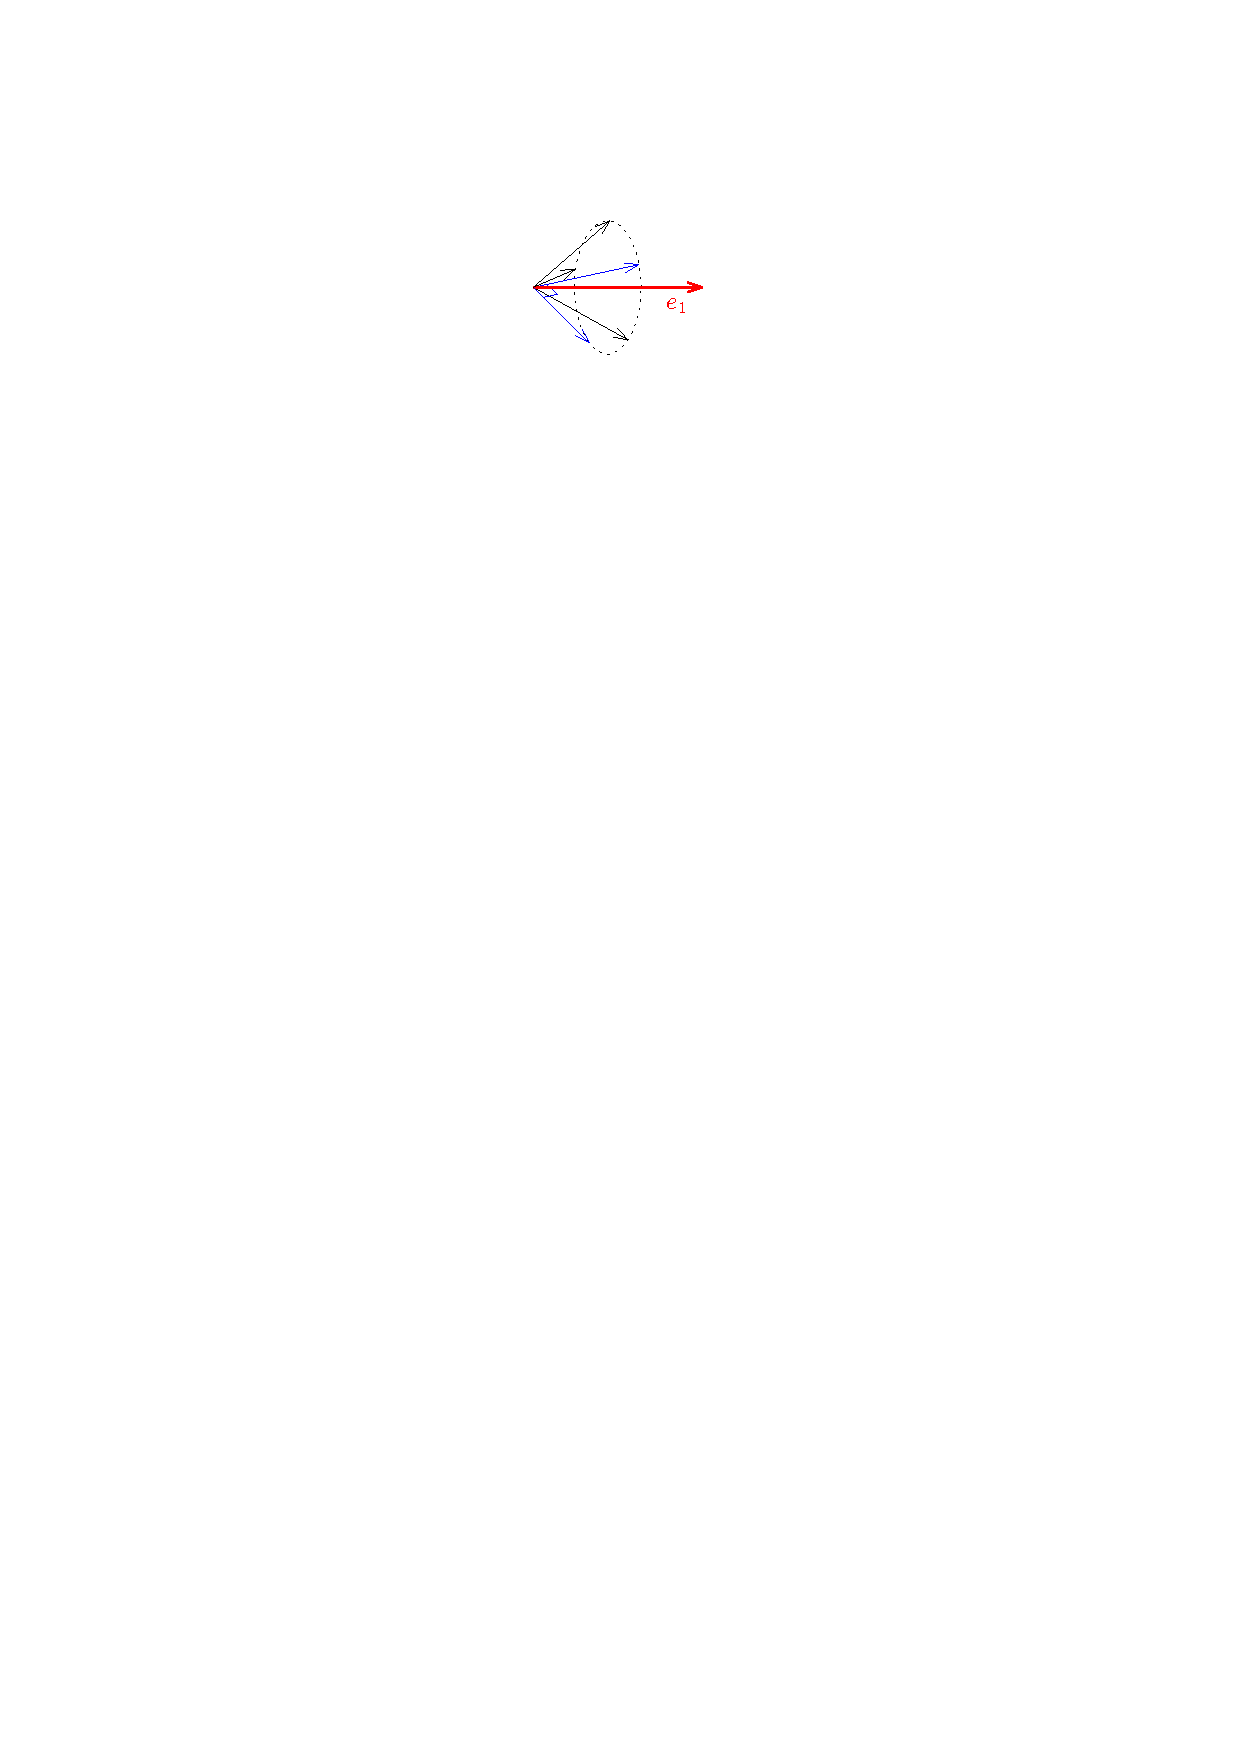
\includegraphics{lovaszovo_paraplicko.pdf}
\end{center}

\df $\vartheta(G) = \min\limits_{\rho\ \text{ONR}} \vartheta(G,\rho)$

Z toho plyne $\vartheta(C_5)\le \sqrt 5$. Kdybychom ještě znali vztah mezi
$\shn(G)$ a $\vartheta(G)$, měli bychom vyhráno. Tuto charakterizaci přináší
následující věta.

\vt $\shn(G) \le \vartheta(G)$

\dk K důkazu věty budeme potřebovat dvě pomocná lemmata.


\lm (O vztahu $\vartheta$ a $\alpha$) Nechť $H$ je graf a $\rho$ nějaká jeho ortonormální reprezentace. Pak $\alpha(H) \leq \vartheta(H, \rho)$.

\dk Nechť $A$ je nějaká nezávislá množina $H$. Zřejmě vektory $\rho(v)$ pro $v \in A$ tvoří ortonormální systém vektorů. Přáli bychom si odhadnout, jak velký bude skalární součin $\sk{\rho(v),e_1}^2$, z čehož nám vztah vyplyne.

Nechť $u$ je libovolný vektor a $b_i$ jsou vektory ortonormální báze. Chceme-li vyjádřit vektor $u$ proti bázi $b_i$, získáme $i$-tou souřadnici skalárním součinem $\sk{b_i,u}$ (můžeme si to představovat tak, že z vektorů $b_i$ složíme matici přechodu). Použijeme-li Pythagorovu větu, získáme:
\begin{align}
	||u||^2 = \sum_{i=1}^d \sk{b_i,u}^2
\end{align}
Pokud aplikujeme tento poznatek na vektory $\rho(v)$ rozšířené na bázi (což jistě lze), a vektor $e_1$, rovnost se změní na nerovnost (nezajímají nás přidané vektory) a s vědomím, že všechny vektory máme ortonormální, získáme:
\begin{align}
	1=||u||^2 \geq \sum_{v\in A}\sk{\rho(v),e_1}^2
\end{align}
Tedy existuje alespoň jeden vrchol $w$, že $\sk{\rho(w),e_1}^2 \leq 1/|A|$ a dosadíme-li do zlomku z definice $\vartheta$, získáme odhad $ \alpha(G) = |A| \leq\vartheta(H,\rho)$, což jsme chtěli dokázat. \qed



\lm (O součinu $\vartheta$) Nechť $H_1$ a $H_2$ jsou grafy, a $\rho_i$ jejich 
ortonormální reprezentace. Potom existuje ortonormální reprezentace $\rho$ 
silného součinu $H_1 \boxtimes H_2$, pro niž platí $\vartheta(H_1 \boxtimes H_2, 
\rho) = \vartheta(H_1, \rho_1) \cdot \vartheta(H_2,\rho_2)$.

\dk Zadefinujme si funkci $\rho$ pro vrcholy $v_i$ následovně:
\begin{align}
	\rho(v) = \rho_1(v_1) \otimes \rho_2(v_2)
\end{align}
Kde operace $\otimes$ je tenzorový součin vektorů, tedy pro $x \in \R^n$ a $y 
\in \R^m$ je výsledek vektor $z \in \R^{mn}$, který obsahuje všechny součiny 
$x_iy_i$. 

Zbývá pouze ověřit, že dělá správnou věc. Podívejme se tedy nejdříve na skalární 
součin:
\begin{align}
	\sk{x \otimes y , x' \otimes y'} = \sk{x,x'} \cdot \sk{y,y'}
\end{align}
Pokud levou a pravou stranu zvlášť rozepíšeme, je vidět, že roznásobením sum 
napravo získáme sumu nalevo a rovnost tedy platí:
\begin{align}
	\sum_{ij} (x_iy_j) \cdot (x_i' y_j') = \left( \sum_i x_ix_i'\right) \left(\sum_j 
	y_jy_j' \right)
\end{align}
Zde již jednoduchou úvahou zjistíme, že $\rho$ je stále ortonormální 
reprezentace: zjevně pro kolmé vektory jsou jejich tenzorové součiny opět kolmé, a všechny vektory si 
zachovají délku $1$. Nyní se stačí podívat, co se stane s $\vartheta$ funkcí, 
rozepišme si ji ted z definice:
\begin{align*}
	\vartheta(H_1 \boxtimes H_2, \rho) &= \max_{v\in V(H_1 \boxtimes H_2)} { 1 
	\over \sk{\rho(v) , e_1}^2} \\
	&= \max_{v\in V(H_1 \boxtimes H_2)} { 1 \over \sk{\rho_1(v_1)\otimes \rho_2(v_2) , e_{11} \otimes e_{12}}^2} \\
	&= \max_{v\in V(H_1 \boxtimes H_2)} { 1 \over \sk{\rho_1(v_1) , e_{11}}^2
		\cdot \sk{\rho_2(v_2) , e_{12}}^2} \\
	&= \max_{v_1\in V(H_1)} { 1 \over \sk{\rho_1(v_1) , e_{11}}^2} \cdot
	  \max_{v_2\in V(H_2)} { 1 \over \sk{\rho_2(v_2) , e_{12}}^2} 
	&= \vartheta(H_1,\rho_1) \cdot \vartheta(H_2, \rho_2)
\end{align*}
A lemma je dokázáno. \qed


\dk (Věty o vztahu $\Theta$ a $\vartheta$)  $$\alpha(G^i) \le \vartheta(G^i) \le \vartheta(G)^i$$
První nerovnost plyne z lemmatu o vztahu $\vartheta$ a $\alpha$. Druhá plyne z
opakovaného použití lemmatu o součinu $\vartheta$.
\qed


\lm (O dvojité kapacitě) $\shn(G + \overline{G}) \ge \sqrt{2|G|}$

\dk Ukážeme, že $\alpha ((G+\overline G)^2) \geq 2|G|$.
\begin{align*}
	V_{G+\overline G} = \{ v_1, ..., v_n, v_1', ..., v_n'\}
\end{align*}

Vezeme graf $(G+\overline G)^2$ a najdeme v něm nezávislou množinu $A$:
\begin{align*}
	A = \left\{\begin{matrix}
		(v_1, v_1'), (v_2, v_2'), \dots \\
		(v_1', v_1), (v_2', v_2), \dots
		\end{matrix}\right\}
\end{align*}

Velikost $A$ je zřejmě $2|G|$ a z definice Shannonovy kapacity dostaneme:
$$\shn(G + \overline{G}) \ge \sqrt{2|G|}$$
\qed



\subsection{Funkční reprezentace grafu}

\df Nechť $G$ je graf, $X$ množina, $\Ft$ těleso a $\F\colon X\rightarrow\Ft$ systém funkcí. Pak pro vrchol $v$ mějme $c_v\in X$ a $f_v \in \F$, že
$f_v: X \to \Ft$ a platí:
\begin{enumerate*}
	\item $f_v(c_v) \neq 0$
	\item $uv \notin E_G \Rightarrow f_u(c_v) = 0$
\end{enumerate*}

\df Dimenzi $\F$ definujeme jako $\dim\L(\{f_v\})$, tedy chápeme funkce
jako vektorový prostor.

\lm(O vztahu $\alpha$ a $\dim\F$) G má reprezentaci $\F$, pak $\alpha(G)
\leq \dim \F$.

\dk Nechť $A$ je nezávislá v $G$. Pak $\{f_a\}_{a\in A}$ je lineárně
nezávislá, stejně jako $\{c_a\}_{a\in A}$. Vyhodnotím reprezentující
funkci v bodech $A$.
\begin{align}
M = \left(
	\begin{matrix}
		f_1(c_1) & f_1(c_2) & \dots \\
		f_2(c_1) & f_2(c_2) & \dots \\
		\vdots &&\\
	\end{matrix}\right)
\end{align}

Matice $M$ bude mít na diagonále nenuly a všude jinde nuly. Tím pádem
jsou její řádky lineárně nezávislé a její dimenze je $|A|$. Navíc zjevně
$\dim M \le \dim\F$.
\qed


\lm(O dimenzi součinu reprezentací) Pokud $G_1$ má reprezentaci $\F_1$,
$G_2$ reprezentaci $\F_2$ nad stejným tělesem, pak $G = G_1 \boxtimes
G_2$ má reprezentaci $\F$,pro kterou platí $\dim\F \leq \dim\F_1 \cdot \dim\F_2$.

\dk Definujeme: 
\begin{align*}
& X = X_1 \times X_2 \\
& c_{(v_1,v_2)} = (c_{v_1}, c_{v_2}) \\
& f_{(v_1, v_2)}((x_1,x_2)) = f_{v_1}(x_1) \cdot f_{v_2}(x_2)
\end{align*}

Ověříme, že výše uvedené je funkční reprezentace a vezmeme si $B_1$ bázi
$\F_1$ a $B_2$ bázi $\F_2$. Pak $\{b_1 \otimes b_2\}_{b_1\in B_1, b_2\in
B_2}$ generuje celý prostor $\F$ a tudíž:
$$
	\dim\F \le |B_1|\cdot |B_2| = \dim\F_1 \cdot \dim\F_2
$$
\qed

\lm(O vztahu $\shn$ a $\dim\F$) G má reprezentaci $\F$, pak $\shn(G)
\leq \dim \F$.

\dk 
$$\shn(G) = \sup_i \alpha(G^i)^{1/i} \leq \sup_i(\dim f.r.(G^i))^{1/i} \leq \sup_i\dim f.r. (G) = \dim f.r.(G)$$

První nerovnost plyne z lemmatu o vztahu $\alpha$ a $\dim\F$, druhá z
lemmatu o dimenzi součinu reprezentací.
\qed


\vt Existuje $G, H$, že $\shn(G+H) > \shn(G) + \shn(H)$

\dk Zvolím $G$ takový, že $V_G={S\choose 3}$, $S = \{1, \dots, s\}$ a $E_G = \{ (A, B): |A\cap B| = 1\}$. 

Reprezentaci vytvoříme nad tělesem $\Ft = \Z_2$, $X = \Z_2^s$:
\begin{align*}
	c_A &= \text{charakteristický vektor } A \\ 
	f_A(x) &= \sum_{a\in A} x_a
\end{align*}

Ověříme, že se jedná o funkční reprezentaci a všimneme si, že každá
funkce $f_A$ je kombinace tří funkcí $b_i(x) = x_i$, přičemž počet funkcí
$b_i$ je $s$.
$$
\dim f.r.(G) \le s \qquad\Rightarrow\qquad \shn(G) \le s
$$

Dále pro $H = \overline G$ zvolíme reprezentaci pro $\Ft = \R$, $X =
\R^s$:
\begin{align*}
	c_A &= \text{charakteristický vektor } A \\ 
	f_A(x) &= (\sum_{a\in A} x_a) - 1
\end{align*}

Opět ověříme, že se jedná o funkční reprezentaci.
$$
\dim f.r.(\overline G) \le s+1 \qquad\Rightarrow\qquad \shn(\overline G) \le s+1
$$

$$\shn(G + \overline G) \ge \sqrt{2{s\choose 3}} > 2s+1 \ge \shn(G) + \shn(\overline G)$$

První nerovnost platí z lemmatu o dvojité kapacitě a ostrou nerovnost
musíme splnit, aby věta platila. Zvolíme si tedy $s \ge 16$.
\qed

\df Obecná poloha vektorů množiny $\check N$ v  $\R^d$ je taková, že libovolná podmnožina velikosti $\leq d$ je lineárně nezávislá.

\df Lokálně obecná poloha vektorů reprezentace v $\R^d$ na grafu $G$ jsou takové vrcholy, že $\rho(\overline{N(v)})$ jsou lineárně nezávislé.

\vt Pro $G$ s $|G| = n$ jsou následující tvrzení ekvivalentní:
\begin{enumerate}
	\item $G$ má ortogonální reprezentaci v $\R^d$ v obecné poloze.
	\item $G$ má ortogonální reprezentaci v $\R^d$ v lokálně obecné poloze.
	\item $G$ je $(n-d)$-souvislý.
\end{enumerate}





\section{Vlastní čísla grafu}

\subsection{Vlastní čísla grafu}


\df Nechť $A$ je čtvercová matice. Potom pokud pro nějaké $\lambda$ a $x$ netriviální platí, že $Ax=\lambda x$ říkáme, že $\lambda$ je vlastní číslo $A$ a $x$ je vlastní vektor příslušící k $\lambda$.

\df Spektrum matice $A$ je množina jejích vlastních čísel. Značíme $\Sp(A) = \{ \lambda_1, \ldots, \lambda_n \}$.

\df Podprostorem generovaným vlastním číslem číslem $\lambda$ rozumíme $V_\lambda = \{u | Au = \lambda u \}$. Geometrická násobnost $\lambda$ je poté dimenze tohoto prostoru $V_\lambda$.

\tv $V_\lambda$ je vektorový prostor.

\dk Stačí dokázat uzavřenost. Pro $u,v\in V_\lambda$ počítejme:
\begin{align}
	A(u+v) = Au + Av = \lambda u + \lambda v = \lambda(u+v)
\end{align}
Tedy i $u+v\in V_\lambda$. \qed

\tv Vlastní čísla matice $A$ lze vypočítat jako kořeny rovnice $\det(A - \lambda \cdot E) = 0$.
\dk Z definice počítejme:
\begin{align}
	Au &= \lambda u \\
	Au - \lambda u &= \vec0 \\
	(A-\lambda) u &= \vec0 \\
	\det(A - \lambda E) &= 0 
\end{align}
Přičemž v posledním kroku využíváme faktu, že pro součin netriviálního vektoru s maticí musí být matice singulární, aby mohl vyjít nulový vektor a tudíž můžeme přejít k determinantu. \qed

\df Polynomu $P_A(\lambda) = \det(A - \lambda \cdot E)$ říkáme charakteristický polynom.

\df Násobnosti kořene $\lambda$ v polynomu $P_A$ říkáme {\it algebraická násobnost}.

\vt Nechť $GN(\lambda)$ a $AN(\lambda)$ značí geometrickou, resp. algebraickou násobnost $\lambda$. Potom platí:
\begin{align}
&GN(\lambda) \geq 1 \Leftrightarrow \lambda \in \Sp(A) \Leftrightarrow AN(\lambda) \geq 1\\
\text{a}\qquad &GN(\lambda) \leq AN(\lambda)
\end{align}
\dk {\it (bez důkazu)}

\df Hermitovská transpozice matice $A$ je matice $A^*$, taková, že $A_{ij}^* = \overline{A_{ji}}$.

\df Matice $A \in \C^{n\times n}$ je {\it normální}, pokud $AA^* = A^*A$.

\vt Matice $A$ má ortonormální bázi složenou z vlastních vektorů právě tehdy, když je $A$ normální.

\dk \begin{description}
	\item \uv{$\Rightarrow$} Nechť $x_i$ jsou vlastní vektory příslušející vlastním číslům $\lambda_i$ tvořící ortonormální bázi. Z ortonormality plyne, že $XX^*=E$, kde $X$ má ve sloupcích $x_i$. Podívejme se nyní jak vypadá matice $X^* A X$:
	\begin{align}
		X^* A X = 
		\underbrace{
		\left(\begin{array}{ccc} &\vdots &\\ \hline \hspace{1cm}& x_j^* & \hspace{1cm}\\ \hline&\vdots& \end{array}\right)}_{=X^*} 
		\underbrace{\left(\begin{array}{c|c|c} \raisebox{5mm}{\ } & &\\ \dots& \lambda_i x_i & \dots\\\raisebox{5mm}{\ }  && \end{array}\right)}_{=AX}
		= \left(\begin{array}{ccc}\lambda_1 &&\bigzero \\ &\ddots & \\ \bigzero&&\lambda_n\end{array}\right)
	\end{align}
	Přičemž druhá matice vznikla ze vztahu $Ax=\lambda x$, přičemž jsme vynásobili všechny vektory naráz díky tomu, že byly v matici. Poslední rovnost plyne z pozorování, že na pozici $ij$ nalezneme výraz $x_j^*\lambda_i x_i = x_j^* x_i \lambda_i$ a protože vektory $x_l$ tvoří ortonormální bázi, jsou nula pokud je $i\neq j$ a jedna jinak.

	Nyní víme, že $X^*AX=D$, kde $D$ je nějaká (konkrétní) diagonální matice. Nyní již snadno vypočteme elementárními úpravami:
	\begin{align*}
		X^* A X = D \quad \Rightarrow \quad AX &= XD \quad \Rightarrow A = XDX^* \\
		A\cdot A^* = XD\underbrace{X^*\cdot X}_ED^*X^* = XDD^*X^*
		&= XD^*DX^* = XD^*\underbrace{X^*\cdot X}_EDX^* = A^*\cdot A
	\end{align*}
	Přičemž jediná finta, kterou jsme použili je, že $DD^* = D^*D$, což je zřejmě pravda, protože jsou to diagonální matice.

	\item \uv{$\Leftarrow$} \todo{gavento} byl jen pochybny naznak
\end{description}

\vt Nechť $A_i \in \C^{n\times n}$ a $\forall i,j$ jsou $A_i$ a $A_j$ normální a $A_iA_j = A_j A_i$. Potom existuje společná ortonormální báze z vlastních vektorů.

\dk \todo{Gavento}

\vt Nechť $A$ je hermitovská matice, tedy $A = A^*$. Potom všechna její vlastní čísla jsou reálná.

\dk Víme, že existuje nějaké $D$ diagonální s vlastními čísly na diagonále a $X$, že $X^*AX = D$. Dále počítáme:
\begin{align}
	D^* = (X^*(AX))^* = (AX)^*X = X^*A^*X = X^*AX = D
\end{align}
A komplexní sdružení tedy nesmí udělat žádnou operaci, tedy jsou vlastní čísla reálná. \qed



\subsection{Moorovy grafy}


Motivací nechť jsou r-regulární grafy bez krátkých cyklů (troj- a 
čtyř-úhelníků). Triviální konstrukce nám dává odhad na počet vrcholů:
\todo{obrázek konstrukce}
\begin{align}
\label{moorova-podminka}
	|V| \geq 1 + r + r(r-1) = r^2 +1
\end{align}

\df Moorův graf je takový $r$-regulární graf bez troj- a čtyř-úhelníků, kde 
platí v (\ref{moorova-podminka}) rovnost.

\vt Moorův graf existuje pro $r=1,2,3,7$, pro $r=57$ se neví a pro žádné další 
$r$ neexistuje.

\dk (Idea) Mějme graf $G$ Moorův a $A$ jeho matici sousednosti. Zapišme druhou 
mocninu $A$ jako stupeň na diagonále a prohozené 0 a 1 jinde a upravme:
\begin{align}
	&A^2 = rE + {\bf0} + {\bf1}(J- A-E) \\
	&A^2 = rE - J - A - E \\
	\label{moorova-matice}&A^2 + A + (1-r)E = J
\end{align}
Dále pro nějaké $\lambda\in \Sp(A)$:
\begin{align}
	\label{moorova-mocnina}A^2 x = AAx = A\lambda x = \lambda A x = \lambda 
	\lambda x = \lambda^2 x
\end{align}
A dosadíme (\ref{moorova-matice}) za $A$:
\begin{align}
	Jx = (A^2 + A + (1-r)E)x = (\lambda^2 + \lambda + (1-r))x
\end{align}
A tedy $(\lambda^2 + \lambda + 1 -r) \in \Sp(J)$. Vlastní čísla matice $J$ 
(matice samých jedniček) ale známe, jsou to $\{0^{(n-1)}, n^{(1)}\}$. Zjevně pro 
$\lambda = r$ vyjde vlastní číslo $n$, je tedy potřeba vyřešit kvadratickou 
rovnici s parametrem $r$:
\begin{align}
	\lambda^2 + \lambda + 1 - r = 0
\end{align}
Jak na to půjdeme? Vyjádříme si $\lambda$ známým vzorečkem pro kořeny:
\begin{align}
	\lambda_{1,2} = \frac{-1\pm \sqrt{1-4(1-r)}}{2} = \frac{-1\pm\sqrt{4r-3}}{2}
\end{align}
Násobnost označíme $m_1, m_2$. Protože stopa matice je suma vlastních čísel 
včetně násobností, platí dále rovnice (protože matice sousednosti $A$ má na 
diagonále vždy nuly):
\begin{align}
	\Tr(A) = r+m_1\lambda_1 + m_2\lambda_2 = 0
\end{align}
Nejdříve
upravíme do formy (násobení dvěma a přeskupení):
\begin{align}
	2r - r^2 + \sqrt{4r-3}(m_1 - m_2) = 0 \label{4-2:rovnice}
\end{align}
Všimneme si, že $r\in\N$, tedy máme dvě možnosti:
\begin{enumerate}
	\item $\sqrt{4r-3} \not\in \Q$: potom $m_1 = m_2$ a tedy $r = 2$.
	\item $\sqrt{4r-3} = s \in \Q$, což implikuje\footnote{Odmocnina z celého čísla je
  vždy celé číslo či iracionální číslo, nikdy zlomek.} $s \in \N$.
  Substitucí $4r - 3 = s^2$ do rovnice \ref{4-2:rovnice} získáme
	$s \in \set{1, 3, 5, 15}$, což dává $r \in \set{1, 3, 7, 57}$.
\end{enumerate}
\qed



\subsection{Silně regulární grafy}


\df Silně regulární graf je d-regulární, $\forall$ hranu $xy\in E$ $\exists!e$
vrcholů $u: ux,uy\in E$ a $\forall$ nehranu $xy\not\in E$ $\exists!f$ vrcholů
$u: ux,uy\in E$.

Abychom mohli zanedbat triviální případy, dodáváme $f>0$ a $G\neq K_n$.
Příkladem silně regulárního grafu je úplný bipartitní graf se stejně velkými
partitami ($e=0$). Nejmenším nebipartitním silně regulárním grafem je
pětiúhelník ($e=0$, $f=1$).

\vt $G$ je silně regulární graf s parametry $d$, $e$, $f$ a $n$ vrcholy. Potom:
\begin{enumerate}
	\item[(a)] Zafixujeme $f$: $e = f-1$; $d = 2f$; $n = 4f+1$
	\item[] {\it nebo}
	\item[(b)] $\exists s \in \Z$, že platí $(e-f)^2-4(f-d) = s^2$ \\
	a výraz \ ${d\over 2fs}((d-1+f-e)(s+f-e)-2f)$ je přirozené číslo
\end{enumerate}

\dk Nechť G je silně regulární, $A$ je jeho matice sousednosti. $(A^2)_{ij} =
e$, pokud $A_{ij} = 1$. Na ostatních souřadnících bude $f$, na diagonále $d$
(to plyne z jednoduchého pozorování počtu sledů délky 2).

$$
A^2 = \left(
	\begin{matrix}
		d & & f & \\
		& d & & e \\
		f & & \ddots & \\
		& e & & d\\
	\end{matrix}\right)
$$

\begin{align}
	A^2 = dI + eA + f(J-I-A) &= fJ + (d-f)I + (e-f)A \\
	A^2 + (f-e)A + (f-d)I &= fJ \\
	\lambda^2 + (f-e)\lambda + (f-d) &\rightarrow \Sp(fJ)\qquad \lambda\in\Sp A
\end{align}

Víme, že vlastní čísla jedničkové matice $J$ jsou $\Sp(J) = \{n, 0^{n-1}\}$.
Proto $\Sp(fJ) = \{fn, 0^{n-1}\}$. Dále víme, že $d$ je vlastním číslem matice
$A$, neboť graf $G$ je $d$-regulární.

\begin{align}
	&d^2 + (f-e)d + (f-d) \in \Sp(fJ) \\
	&d^2 + (f-e)d + (f-d) = fn \\
\end{align}
\begin{align}
	&\lambda \in \Sp(A) - \{d\} \Rightarrow \lambda^2 + (f-e)\lambda + (f-d) = 0 \\
	&\lambda_{1,2} = {e-f \pm \sqrt{(f-e)^2-4(f-d)} \over 2} \qquad \sqrt{(f-e)^2-4(f-d)} = s
\end{align}

$$\lambda_1 = {e-f+s\over 2}\qquad\qquad \lambda_2 = {e-f-s\over 2}$$

Matice $A$ má vlastní čísla $d$ (1-násobné), $\lambda_1$ ($p$-násobné) a
$\lambda_2$ ($q$-násobné).

\begin{enumerate}
	\item[(1)] $1 + p + q = n$ (celkový počet vlastních čísel)

	\item[(2)] $d + p\lambda_1 + q\lambda_2 = \Tr A = 0$ (stopa\footnote{Stopou (čtvercové) matice rozumíme součet čísel na diagonále. Je známo, že součet vlastních čísel (včetně násobností) je roven stopě matice. Značíme ji $\Tr A$.} matice $A$ je 0) \\
	$d + p\left({e-f+s\over 2}\right) + q\left({e-f-s\over 2}\right) = 0$ \\
	$d + \left({p+q\over 2}\right)(e-f) + \left({s\over 2}\right)(p-q) = 0$

	\item[(3)] $d^2 + p\lambda_1^2 + q\lambda_2^2 = \Tr A^2 = nd$ (vlastní čísla matice $A^2$ jsou druhé mocniny vlastních čísel matice $A$).
\end{enumerate}

\begin{enumerate}
	\item[(a)] $s\not\in Q \Rightarrow p = q$ \quad $d + p(e-f) = 0 \Rightarrow p = {d\over f-e} \Rightarrow (f-e)|d$ \\
	$f-e > 0$ \quad $n = 1 + 2p = 1 + {2d\over f-e}$ \quad (z rovnice (1))

	Pokud $f-e = 1$, pak $e = f-1$ (což chceme). \\
	Pokud $f-e = 2$, pak $n = 1+d$ a $G = K_{d+1}$, ale úplné grafy jsme si zakázali. \\
	Pokud $f-e > 2$, pak $n < 1+d$, což je nesmysl.

	$e = f-1 \quad\Rightarrow\quad n = 2d+1$ \\
	$d^2 + d + (f-d) = f(2d+1) \quad\Rightarrow\quad d = 2f \quad\Rightarrow\quad n = 4f+1$

	\item[(b)] $s\in\Q\Rightarrow s\in\N$ \\
	\todo Prý pokračování na cvičení, nemůžu ho ale najít. Já taky ne. \\
	$$p = {d\over 2fs}\left((d-1+f-e)(s+f-e)-2f\right) \in \N$$
\end{enumerate}
\qed


\vt (Friendship theorem) Nechť $G$ je graf, jehož každé dva vrcholy mají právě jednoho společného souseda. Pak v $G$ existuje vrchol stupně $n-1$.

Friendship theorem tedy tvrdí, že takový graf musí vypadat jako \uv{mlýn}.

\begin{center}
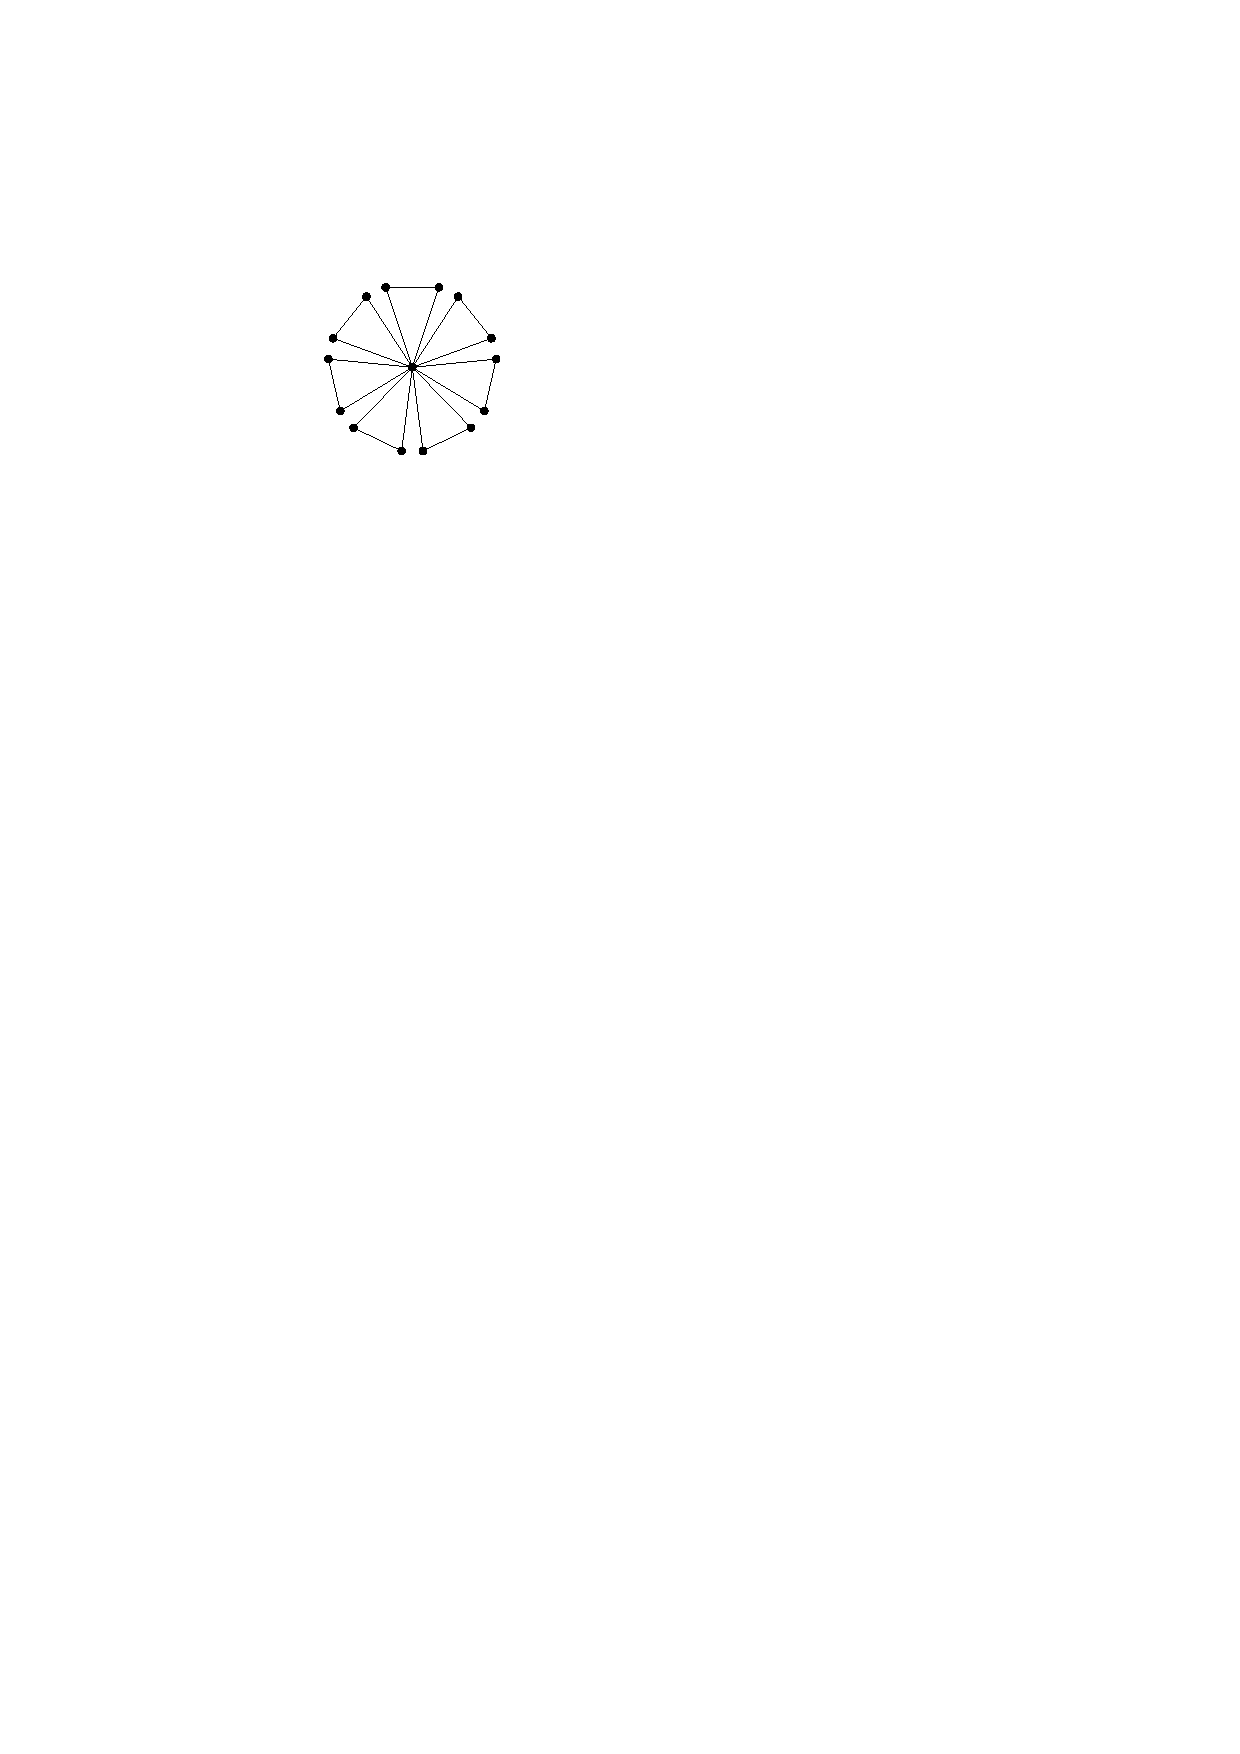
\includegraphics{friendship.pdf}
\end{center}

\dk Nejprve si připomeňme, co jsou to konečné projektivní roviny.

\df Konečná projektivní rovina je množina bodů a přímek, že:
\begin{enumerate}
	\item Každé dvě přímky sdílejí právě jeden bod.
	\item Každé dva body spojuje právě jedna přímka.
	\item Existují 4 body a žádná přímka neprotíná více než dva z nich.
\end{enumerate}

Nyní si označme symbolem $N(v)$ množinu sousedů vrcholu $v$. Všimneme si, že
sousedství pro náš graf přesně odpovídají přímkám v KPR a body jsou body. Protože ale třetí
podmínka by znamenala, že naše věta neplatí, budeme si přát, aby to KPR nebyla
-- pak snadno najdeme vrchol, který je spojený s každým dalším.

Pro spor tedy předpokládejme, že graf KPR je. Protože v KPR mají všechny přímky stejnou mohutnost, je také $d$-regulární. Navíc každé $u,v$ má právě jednoho společného souseda, což znamená, že $G$ je silně regulární s parametry  $e=f=1$.

Podle předchozí věty to ověříme: možnost (a) nastat nemůže, protože $e=f$.
Počítejme tedy, že nastala možnost (b). Protože je to KPR řádu $m$, tak $d=m+1$ a $n=m^2 + m + 1$.
\begin{align}
	(e-f)^2 - 4(f-d) = 0^2 - 4 - 4(m+1))= s^2 \\
	4m = s^2 \\
	s=2\sqrt m 
\end{align}
A ověříme celočíselnost polynomu $p$ s tím, že $t:=s/2=\sqrt m$, tedy $s=2t$ a $m=t^2$:
\begin{align}
	p &= {d \over 2fs} ((d-1+f-e)(s+f-e)-2f) \\
	&= {m+1 \over 4t} ((m+1+0)(2t+0)-2)\\
	&= {(t^2 + 1)(t^3-1) \over 2t}
\end{align}
Což má být přirozené číslo. To je pravda zřejmě jenom pro $t=1$, tedy $n=3$ a pokud náš graf není trojúhelník, jde to spor. Pokud to trojúhelník je, splňuje žádanou vlastnost triviálně. \qed



\subsection{Rayleighův princip a proplétání}


\vt (Rayleighův princip) Nechť $A$ je matice $n\times n$ s ortonormální bazí z vlastních 
vektorů $x_i$ a vlastními čísly $\lambda_1 \geq \lambda_2 \geq\dots\geq\lambda_n$. Potom:
\begin{enumerate}
\item $x \in\sk{x_1,\dots,x_k} \Rightarrow x^*Ax\ge \lambda_kx^*x$
\item $x \in\sk{x_k,\dots,x_n} \Rightarrow x^*Ax\le \lambda_kx^*x$
\end{enumerate}

\dk $x \in\sk{x_1,\dots,x_k} \Rightarrow x = \sum_{i=1}^k \alpha_ix_i$
\begin{align*}
	x^*Ax &= x^*(Ax) = x^*\left(A\cdot\sum_{i=1}^k\alpha_ix_i\right) = x^*\left(\sum_{i=1}^k\alpha_iAx_i\right) = x^*\left(\sum_{i=1}^k\alpha_i\lambda_ix_i\right) = \\
	&= \sum_{i=1}^k\alpha_i\lambda_ix^*x_i = \sum_{i=1}^k\alpha_i\lambda_i\left(\sum_{j=1}^k \alpha_jx_j\right)^*x_i = \sum_{i=1}^k \alpha_i\lambda_i(\alpha_ix_i)^*x_i = \\
	&= \sum_{i=1}^k \lambda_i\underbrace{\alpha_i\overline{\alpha_i}}_{\ge 0} \ge \sum_{i=1}^k \lambda_k\alpha_i\overline{\alpha_i} = \lambda_k\sum_{i=1}^k \alpha_i\overline{\alpha_i} = \lambda_kx^*x
\end{align*}

Poslední rovnost plyne z následujícího:
\begin{align*}
	 \lambda_kx^*x = \left(\sum_{i=1}^k \alpha_ix_i\right)^*\left(\sum_{i=1}^k \alpha_ix_i\right) = \sum_{i=1}^k \alpha_i\overline{\alpha_i}
\end{align*}

Druhou nerovnost dokážeme analogicky. \qed


\vt (Věta o proplétání) Nechť $A$ a $B$ jsou matice takové, že $B$ vznikla z $A$ 
vymazáním nějakého řádku a sloupce. Potom pro vlastní čísla $\lambda_i,\mu_i$ 
matic $A,B$ platí:
\begin{align}
	\lambda_1 \geq \mu_1 \geq \lambda_2 \geq \dots\geq \mu_{n-1} \geq \lambda_n
\end{align}

\dk Dokazujeme $\lambda_k \geq \mu_k \geq \lambda_{k+1}$. Označme $x_i$ 
a $y_i$ vlastní vektory matic $A$ a $B$.  Zaveďme následující vektorové 
podprostory $\C^n$ (ačkoli druhý z nich nemá dostatek složek, můžeme mu jednu 
nulovou přidat a nic se nestane):
\begin{align}
S_1 := \L\{x_k, \dots, x_n\} \subseteq \C^n \\
S_2 := \L\{y_1, \dots, y_k\} \subseteq \C^n
\end{align}
Zřejmě $\dim(S_1) + \dim(S_2) = (n-k+1) + k > n$, tedy $\exists x \in S_1\cap S_2$. Použijeme 
Reileighův princip pro oba prostory a máme:
\begin{align}
	\mu_k \leq \frac{y^*By}{y^*y} = \frac{x^*Ax}{x^*x} \leq \lambda_k
\end{align}
Stačí ukázat, že $\mu_k \geq \lambda_{k+1}$ -- to je ale snadné, stačí vzít $-A$ 
a $-B$, čímž se obrátí znaménka vlastních čísel a nerovnosti. \qed

\vt (Věta o proplétání při násobení maticí) Nechť $A$ je symetrická čtvercová matice 
s vlastními čísly a vektory $\lambda_i$ a $x_i$, $S$ reálná matice, že $S^TS=I$.  
Definujeme $B := S^TAS$ a označíme vlastní čísla a vektory matice $B$ jako 
$\mu_i$ a $y_i$. Potom $\mu_i$ proplétají $\lambda_i$ a pokud navíc $\mu_i = 
\lambda_i$ pro nějaké $i$, tak $Sy_i$ je vlastní vektor $A$ příslušící vlastnímu 
číslu $\lambda_i$.

\dk Použijeme Rayleighův princip podobně jako v předchozím tvrzení. Všimneme 
si, že:
\begin{align}
	x \in \L\{ S^Tx_k, \dots, S^Tx_{n}\}^\perp \Leftrightarrow
	Sx \in \L\{ x_k, \dots, x_{n}\}^\perp
\end{align}
Stačí si opět vzít vhodný prvek $x$ z průniku:
\begin{align}
	x \in \L\{ S^Tx_k, \dots, S^Tx_{n}\}^\perp \cap \L\{y_1, \dots, y_k\}
\end{align}
A můžeme použít Reileighův princip:
\begin{align}
	\lambda_k \geq \frac{(Sx)^TASx}{(Sx)^TSx} = \frac{x^TBx}{x^Tx} \geq \mu_k \\
\end{align}
Navíc platí, že pokud $\lambda_i = \mu_i$, potom:
\begin{align}
	\frac{x^TBx}{x^Tx} = \lambda_i \quad\Rightarrow\quad x^TBx=x^Tx\lambda_i 
	\quad\Rightarrow\quad Bx = \lambda_i x
\end{align}
A $x$ je vlastní vektor příslušící $\lambda_i$, jak jsme chtěli dokázat.\qed

\df $A$ je bloková matice s bloky velikosti $x_1, \dots, x_m$. Kvocient $A$ je matice $B^{m\times m}$, kde $b_{i,j} = $ průměr hodnot $A_{i,j}$.
\begin{align*}
	A = \left(\begin{matrix}
		A_{1,1} & A_{1,2} & \dots \\
		A_{2,1} & A_{2,2} & \dots \\
		\vdots & \vdots & \ddots 
		\end{matrix}\right)
	\qquad
	\qquad
	B = \left(\begin{matrix}
		b_{1,1} & b_{1,2} & \dots \\
		b_{2,1} & b_{2,2} & \dots \\
		\vdots & \vdots & \ddots 
		\end{matrix}\right)
\end{align*}

\vt (Věta o proplétání kvocientu) Pokud $B$ je kvocient $A$, pak vlastní čísla
$B$ proplétají vlastní čísla $A$.

\dk Mějme $\widetilde S$ matici incidence blokové $A$:
\begin{align*}
	\widetilde S = \left(\begin{array}{llll}
		\framebox[3em][c]{1} & & & \hfil\bigzero \\
		& \framebox[4em][c]{1} & & \\
		\bigzero & & \framebox[2em][c]{1} & \\
		& & & \framebox[1em][c]{1}
		\end{array}\right)
\end{align*}

\begin{align*}
	& \widetilde S\cdot\widetilde S^T = \text{diagonální matice } (x_1, x_2, \dots, x_m) = D \\
	& S := \widetilde S \cdot D^{-{1\over2}} \\
	& \widetilde B = S^TAS
\end{align*}

Kromě toho platí:
\begin{align*}
	& S^TS = I
	& B = D^{-{1\over2}}\widetilde BD^{-{1\over2}}
\end{align*}

Tedy $B$ je matice podobná $\widetilde B$ a má stejná vlastní čísla. Matice
$\widetilde B$ proplétá matici $A$, což plyne z věty o proplétání při násobení
maticí. \qed




\section{Náhodné procházky}

\subsection{Markovovské řetězce}


\df Markovovský řetězec je orientovaný graf s váženými hranami takový, že
výstupní stupeň každého vrcholu je 1. Markovoský řetězec často reprezentujeme
maticí přechodu $P$, kde $P_{ij}$ udává pravděpodobnost, že ze stavu $i$
přejdeme do stavu $j$.

\df Distribuce $\pi$ je vektor, jehož součet je 1 a kde $p_i$ určuje
pravděpodobnost, že se nacházíme ve stavu $i$.

\pzn Máme-li distribuci $\pi$ a provedeme jeden krok na Markovovském řetězci s
maticí přechodu $P$, dostaneme novou distribuci $\pi\cdot P$.

\df Markovovský řetězec je reversibilní, existuje-li distribuce $\pi$
t. že $\pi_i\cdot P_{ij} = \pi_j\cdot P_{ji}$.

\lm Markovovský řetězec je reversibilní $\Leftrightarrow$ je odvozen z váženého neorientovaného grafu.

\dk 
\begin{itemize}

\item[\uv{$\Leftarrow$}]
Zvolíme si $\pi$ následovně a ukážeme, že splňuje reversibilní podmínku:
\begin{align*}
& \pi_v = {\deg v\over \sum_{u\in V(G)} \deg u} & P_{ij} = {w_G(i,j)\over \deg i} \\ 
\end{align*}
\begin{align*}
\pi_i P_{ij} &= \pi_i {w_G(i,j)\over \deg i} = {w_G(i,j)\over \sum_{u\in V(G)}\deg u} \\
\pi_j P_{ji} &= \pi_j {w_G(j,i)\over \deg j} = {w_G(j,i)\over \sum_{u\in V(G)}\deg u}
\end{align*}

\item[\uv{$\Rightarrow$}]
Zvolíme váhu $w(i,j) = P_{i,j}\pi_i = P_{j,i}\pi_j = w(j,i)$ a dostaneme vážený
neorientovaný graf.
\qed
\end{itemize}

\df $\pi$ je stabilní distribuce\footnote{Někdy též zvaná \uv{stacionární}.},
je-li $\pi\cdot P = \pi$. Jinak řečeno, stabilní distribuce se po provedení
kroku nezmění.

\vt Pro $G$ neorientovaný souvislý platí: $\forall \rho$ počáteční distribuci
$\set{ \rho P_G^k }_k$ konverguje $\Leftrightarrow$ $G$ není bipartitní.

\dk \begin{description}
	\item \uv{$\Rightarrow$} Pokud je $G$ bipartitní, stačí jako protipříklad vzít distribuci, která začíná jenom v jedné partitě. Pak každým pronásobením matice se celá distribuce přesune do druhé partity, protože nemá kam jinam. Zjevně tedy nekonverguje k jedinému rozložení.
	\item \uv{$\Leftarrow$} Prvně si vyjádříme distribuci jako lineární kombinaci vlastních vektorů matice $P_G$ (to lze, protože tvoří ortonormální bázi). Tedy $\rho = \sum_i a_ip_i$. Dále si vyjádříme distribuci po $k$ iteracích:
  \todo{distribucí násobíme zleva, dále (levým) vlastním vektorem 1 není vektor jedniček,
        ale stabilní distribuce $\pi$ \dots}
	\begin{align}
		P_G^k\rho = P_G^k\sum_ia_ip_i = \sum_iP_G^ka_ip_i
	\end{align}
	Protože $p_i$ je vlastní vektor $P_G$, tak $P_Gp_i = \lambda_ip_i$:
	\begin{align}
		\sum_i\lambda_i^ka_ip_i
	\end{align}
  \todo{$P$ není matice sousednosti\dots}
	Nyní si všimneme, že protože graf není bipartitní, tak $\lambda_1 \neq -\lambda_n$ a největší vlastní číslo distribuce je $1$, protože matice $P_G$ má řádkové i sloupcové součty konstantní $1$ a zároveň je $1$ má vlastní vektor samých jedniček. Tedy pro $i > 1$ platí $|\lambda_i| < 1$. Dejme nyní výraz do limity a všimneme si, že suma jde k nule díky tomu, že jediný člen závislý na $k$ je $\lambda_i$:
	\begin{align}
		\lim_{k\to \infty}\left(\lambda_1^ka_1p_1 + \sum_{i>1}\lambda_i^ka_ip_i\right) = a_1p_1 = \pi
	\end{align}
	Tedy máme stabilní distribuci, protože $a_1p_1$ jsou po celou dobu konstantní.
\end{description}

\vt Nechť $\rho$ je distribuce na vrcholech grafu a $\mu=\max\{\lambda_i,-\lambda_n\}$. Pak po $t$ krocích platí, že $\|P_G^t\rho - \pi\|_1 \leq \mu^t\sqrt{n}$, tedy distribuce konverguje relativně rychle.

\dk Z předchozího důkazu víme, že $\rho = p_ia_i + \sum_{i>1} \lambda_i^ta_ip_i$ a \todo{vec}.

Pusťme se do odhadu naší odchylky, prozatím však v $L_2$ normě.

\begin{align}
	\|P_G^t\rho - \pi\|_2^2 = \left\|\sum_{i > 1} \lambda_ia_ip_i\right\|_2^2 = \sum_{i>1}\lambda_i^{2t}\|a_ip_i\|_2^2
\end{align}
Nyní si zjednodušíme práci a do sumy zahrneme i první člen. Navíc odhadneme $\lambda_i$ největšším vlastním číslem $\mu$ (mocnina u $\lambda_i$ je sudá!).
\begin{align}
	\leq \mu^{2t}\sum_i\|a_ip_i\|_2^2 = \mu^{2t}\|\rho\|_2^2 \leq \mu^{2t}
\end{align}
Nyní stačí výraz odmocnit a vzpomenout si na analýzu, čímž víme, že $\|x\|_1 \leq \|x\|_2 \cdot \sqrt n$ a máme nerovnost:
\begin{align}
	\|P_G^t\rho - \pi\|_2 &\leq \mu^{t} \\
	\|P_G^t\rho - \pi\|_1 &\leq \mu^{t} \sqrt n
\end{align}
Což jsme chtěli dokázat. \qed


\input{5-2-konvergence-procesu.tex}


\section{Expandéry}

\subsection{Expanze}


\df
\begin{itemize}
	\item $E(S,T) = \{$ hrany mezi $S$ a $T$ $\}$
	\item $e(S,T) = |E(S,T)|$
	\item $e(S) = $ počet hran uvnitř $S$
	\item vrcholová expanze $h_v(G) = \min\limits_{S\subseteq V, |S|\le {n\over 2}}
                                        {|N(S) \setminus S| \over |S|}$
	\item hranová expanze $h(G) = \min\limits_{S\subseteq V, |S|\le {n\over 2}} {e(S,\bar S) \over |S|}$
\end{itemize}

\poz $h_v(G) \le h(G) \le d . h_v(G)$

\df 
\begin{itemize}
	\item Rodina expanderů $\{G_i\}_\infty$\quad$2^i \ge |G_i| \ge i: h(G_i) \ge \varepsilon$, $G_i$ je $d$-regulární.
	\item Spectral gap $= d - \max\{\lambda_2,-\lambda_n\}$
	\item Spektrální expanze $= d - \lambda_2$
	\item $\lambda = \max\{\lambda_2,-\lambda_n\}$
\end{itemize}

\vt ${1\over 2}(d-\lambda_2) \le h(G) \le \sqrt{d(d-\lambda_2)}$ (G je $d$-regulární graf).

\dk (Jen první nerovnost, druhá je bez důkazu). Sporem: nechť $S$ je množina
vrcholů s malou hranovou expanzí.

Pro $x \bot (1,1,\dots,1)$ platí $\lambda_2 \ge {x^TAx\over x^Tx}$ (Raileighův
princip). Zvolíme $x = (n-s)1_S - s1_{\bar S}$, kde $s = |S|$ a $1_S$ je
charakteristický vektor množiny $S$.

$$x^Tx = (n-s)^2s + s^2(n-s) = s(n-s)n$$
$$x^TAx = \sum_{(a,b)\in E} 2x_ax_b = 2(n-s)^2e(S)-2s(n-s)e(S,\bar S) + 2s^2e(\bar S)$$

Platí $ds = 2e(S) + e(S,\bar S)$, neboť $ds$ odpovídá počtu konců hran v $S$. Analogicky $d(n-s) = 2e(\bar S) + e(S,\bar S)$ pro $\bar S$. Z toho si vyjádříme $e(S)$ a $e(\bar S)$ a dosadíme do rovnice výše:

$$x^TAx = -e(S,\bar S)n^2 + (n-s)ds(n-s+s) = (n-s)dsn - e(S,\bar S)n^2$$
$$\lambda_2 \ge {(n-s)dsn - e(S,\bar S)n^2 \over s(n-s)n} = d - {n\over n-s}\cdot{e(S,\bar S)\over s}$$
$$d-\lambda_2 \le {n\over n-s} \cdot {e(S,\bar S)\over s} \le 2\cdot{e(S,\bar S)\over s} = 2h(G)$$
\qed

\lm Pro náhodný d-regulární graf skoro jistě platí $\lambda \le 2\sqrt{d-1} + O(1)$. Bez důkazu.



\subsection{Mixing lemma}


\vt (Mixing lemma) $\forall G$ $d$-regulární, $\forall S,T \subseteq V, S\cap T = \emptyset: |e(S,T) - {d\cdot|S|\cdot|T|\over n}| \le \lambda d\cdot\sqrt{|S|\cdot|T|}$

\dk Buďte $\chi_S, \chi_T$ charakteristické vektory $S$ a $T$. $u = (1,1,\dots)$ je první vlastní vektor. $\chi_S^\bot$ značí vektor kolmý na $u$.

$${\sk{\chi_S \cdot u} \over \|u\|^2} = {|S|\over n} \qquad\Rightarrow\qquad \chi_S = u\cdot {|S|\over n} + \chi_S^\bot \qquad\qquad \chi_T = u\cdot {|T|\over n} + \chi_T^\bot$$

$$e(S,T) = \sum_{i\in S, j\in T} A_{ij} = \chi_T^TA\chi_S = \underbrace{{|S|\cdot |T| \over n^2} \underbrace{u^TAu}_{d\|u\|^2=dn}}_{d\cdot |S|\cdot |T|\over n} + \xttt A\chi_s^\bot$$

Zbývá dokázat, že $|\xttt A\chi_S^\bot| \le \lambda\cdot\sqrt{|S|\cdot |T|}$.

$$|\xttt A\chi_S^\bot| \le \|\xttt \| \cdot \|A\chi_S^\bot\| \le \|\xttt\|\cdot\lambda\cdot\|\chi_S^\bot\|$$

První nerovnost plyne z toho, že skalární součin dvou vektorů (tedy součin
jejich délek a sinu úhlu, který svírají) je vždy nejvýš roven součinu jejich
délek. Druhá nerovnost plyne z toho, že si $\chi_S^\bot$ můžu vyjádřit jako
lineární kombinaci vlastních vektorů $A$:

$$\chi_S^\bot = \sum_{i=2}^n y_i\alpha_i$$

Pro každý vlastní vektor $y_i$ můžu nahradit matici $A$ vlastním číslem
$\lambda_i$ (pak bude zachována rovnost) a tím spíš můžu nahradit matici $A$
největším vlastním číslem, což je v našem případě $\lambda =
\max\{\lambda_2,-\lambda_n\}$, abych zachoval nerovnost.

$$\|\chi_S\|^2 = |S| \qquad\Rightarrow\qquad \|\xttt\| \le \sqrt S$$
$$\|\chi_T\|^2 = |T| \qquad\Rightarrow\qquad \|\chi_S^\bot\| \le \sqrt T$$

$$|\xttt A\chi_S^\bot| \le \lambda\cdot\sqrt{|S|\cdot |T|}$$
\qed


\input{6-3-zvetsovani-expanze.tex}


\section{Perfektní kódy}

Perfektní kódy jsou v jistém smyslu ty nejlepší samoopravné kódy, konkrétně mají vlastnost, že žádná slova z abecedy nezůstávají nevyužita. Cílem našeho snažení bude ukázat větu, která tyto kódy charakterizuje ve smyslu, při jakých parametrech může být kód perfektní. Začneme připomenutím základních pojmů, vyslovíme a dokážeme Lloydovu větu o nutné podmínce a z ní následně dokážeme (v současné podobně spíše nastíníme) kýženou charakterizaci.

\medskip
\subsection{Samoopravné kódy}



\df Samoopravný kód $C$ s parametry $(n, M)_q$ nad abecedou $A$ je podmnožina $A^n$, kde $|A|=q$ a $|C|=M$. Prvkům množiny $C$ říkáme kódová slova.

Nejčastěji $A$ je konečné těleso $GF(q)$ o $q$ prvcích nebo $A=\{0, \dots, q-1\}$. Pokud $C$ je vektorový podprostor nad tělesem $A$, pak $C$ nazýváme lineárním kódem. Množinu $A^n$ navíc vybavíme Hammingovou metrikou $d(~,~)$. Pro dvě slova $x, y \in A^n$ se složkami $x_i$ resp. $y_i$ platí $$d(x, y)=|\{i~|~x_i\neq y_i\}|.$$ Minimální vzdálenost kódu je pak definována jako $d=\min_{x \neq y \in C} d(x, y)$. Mluvíme pak o $(n, M, d)_q$ kódu. 

Chceme, aby kód měl co největší minimální vzdálenost (při co největší mohutnosti). To souvisí s tím, že pokud vysíláme kódové slovo $c \in C$, může během přenosu dojít k chybám (uvažujeme pouze změnu složky nikoliv zkrácení délky) a druhá strana přijme slovo $y= c + e$, kde $e$ je chybové slovo. Příjemce se pak snaží chybu detekovat a případně opravit $y$ na nejbližší kódové slovo $c' \in C$ (vše je měřeno Hammingovou metrikou). Pokud kódová slova budou co nejdále od sebe, je detekce a oprava $y$ na správné kódové slovo $c$ (tj. $c=c'$) více pravděpodobná. Přesněji pokud počet chyb (což je počet nenulových složek chybového slova $e$) je $\leq d-1$ je možné chybu detekovat (přijmeme-li nekódové slovo, víme, že nastala chyba). Pokud pokud počet chyb je $\leq \lfloor\frac{d-1}{2}\rfloor=:t$ je možné chybu opravit. Označme $N_t(c)=\{x\in A^n~|~d(c, x)\leq t\}$ okolí slova $c$ do vzdálenosti $t$. Vidíme, že okolí $N_t(c)$ pro všechna $c\in C$ jsou disjunktní, kde $C$ má minimální vzdálenost $d$ a $t$ je definováno výše. 





%\df Kód $C$ je $t$-perfektní, pokud opravuje $t$ chyb a navíc úplně pokrývá svou nosnou množinu $M$.

\tv(Hammingův odhad) Mějme $(n, M, d)_q$ kód $C$. Označme $t=\lfloor\frac{d-1}{2}\rfloor$. Pak
\begin{align*}
	|C| \leq { q^n \over \sum_{i=0}^t \binom{n}{i} (q-1)^i }
\end{align*}

\dk Stačí si uvědomit, že okolí jsou disjunktní a obsahují všechny stejně slov (zde nezáleží na středu okolí). Dostáváme tak: 
$$q^n\geq \sum_{c\in C} |N_t(c)|=M\cdot \sum^{t}_{i=0} \binom{n}{i}(q-1)^i.$$
\qed

\df Kódy, která nabývají rovnosti v Hammingově odhadu nazýváme perfektními.

Nyní si ukážeme základní příklady perfektních kódů. Mezi ty triviální patří totální $(n, q^n, 1)$ kód obsahující všechna slova z $A^n$, opakovací $(n, 2, n )$ kód pro lichou délku $n$ a jednoprvkový kód. 

Každý lineární kód můžeme popsat jeho bází. Generující matice $G$ o rozměrech $k \times n$ lineárního $(n, q^k)$ kódů $C$ nad $GF(q)$ má v řádcích zapsanou jeho bázi. Kontrolní matice lineárního kódu $C$ je taková matice $H$ o rozměrech $(n-k) \times n$, že $c\in C \Leftrightarrow Hc^T=0$. Platí $HG^T=0$. Lineární kód můžeme jednoznačně popsat jeho generující nebo kontrolní maticí.

\df Hammingův kód $\mathcal{H}(r, q)$ je určen svojí kontrolní matici o rozměrech $r \times \frac{q^r-1}{q-1}$, která obsahuje ve sloupcích všechny po dvou lineárně nezávislé vektory nad $GF(q)$ délky $r$. Kód $\mathcal{H}(r, q)$ je $1$-perfektní $(\frac{q^r-1}{q-1}, \frac{q^r-1}{q-1}-r, 3)_q$ lineární kód.

\df Uvažme matici $G'=(I_{12}~|~Q)$, kde $Q$ je doplněk matice sousednosti dvacetistěnu. Matice $G'$ generuje $(24, 12, 8)_2$ kód $\mathcal{G}_{24}$ nad $GF(2)$. Vynecháním libovolné fixní souřadnice kódových slov v $\mathcal{G}_{24}$ obdržíme $(23, 12, 7)_2$ kód $\mathcal{G}_{23}$. Kód $\mathcal{G}_{23}$ se nazývá binární Golayův $3$-perfektní kód.

\df Uvažme matici $G=(I_6~|~Q)$, kde 
\begin{displaymath}
Q= \left(
\begin{array}{ccccc}
1& 1 & 1 & 1 &  1\\
0& 1 & 2 & 2 &  1\\
1& 0 & 1 & 2 &  2\\
2& 1 & 0 & 1 &  2\\
2& 2 & 1 & 0 &  1\\
1& 2 & 2 & 1 &  0\\
\end{array}
\right).
\end{displaymath}

Matice $G$ generuje $(11, 6, 5)_3$ kód $\mathcal{G}_{11}$ nad $GF(3)$. Kód $\mathcal{G}_{11}$ se nazývá ternární Golayův $2$-perfektní kód. 

\subsection{Lloydova věta}
Nyní směřujeme k charakterizující větě, která říká, že ve skutečnosti žádné jiné perfektní kódy než výše uvedené nad abecedou mohutnosti mocniny prvočísla neexistují. Důkaz, který uvedeme je kombinatorický. Jádro důkazu spočívá v důkazu Lloydovy věty, která dává silné omezení na existenci perfektních kódů. 



\vt Definujme Lloydův polynom v proměnné $x$ stupně $t$

\begin{displaymath}
	L_t(x) = \sum_{j=0}^t(-1)^j(q-1)^{t-j}\binom{x-1}{j}\binom{n-x}{t-j}
\end{displaymath}
Pokud existuje $t$-perfektní kód délky $n$ nad abecedou mohutnosti $q$, pak $L_t(x)$  má $t$ různých celočíselných kořenů mezi $1$ a $n$.

K důkazu Lloydovy věty budeme potřebovat vlastnosti vzdálenostně regulárních grafů. 

\subsection{Vzdálenostně regulární grafy}


\df Uvažme graf $\Gamma=(V,E)$, že $V(G) = A^n$ a hrana mezi vrcholy $u,v$ vede právě tehdy, když $d(u, v) = 1$, tedy liší se právě v jedné souřadnici. Kód v grafu $\Gamma$ příslušející kódu $C$ je pak podmnožina vrcholů, které odpovídají kódovým slovům $C$.

Graf $\Gamma$ je speciálním případem vzdálenostně regulárního grafu. Poznatky z této sekce na závěr aplikujeme právě na $\Gamma$. Po celou dobu této podkapitoly pracujeme pouze s vzdálenostně regulárními grafy.

\df Graf $G$ je vzdálenostně regulární, pokud existují konstanty $s_{hij}$ tak, že  pro $\forall u,v\in V(G), d(u,v) = j$ je $$|\{w: d(u,w) = h, d(w,v) = i\}| = s_{hij}.$$

\poz $|i-j| > h \Rightarrow s_{hij} = 0$ (plyne z trojúhelníkové nerovnosti), $k = s_{110}$ je počet sousedů libovolného vrcholu v $k$-regulárním grafu. 

\lm Platí $$z_{mi} = z_{m-1,i-1} \cdot s_{1,i-1,i} + z_{m-1,i} \cdot s_{1,i,i} + z_{m-1,i+1} \cdot s_{1,i+1,i},$$ kde $z_{mi}$ značí počet sledů délky $m$ mezi vrcholy ve vzdálenosti $i$.

\dk $z_{00} = 1$, jinak $z_{0i} = 0$. Dále dokážeme indukcí pro $m \ge 1$ a $i
\ge 1$. $s_{1,i,j}$ je nenulové pouze pro $i \in \{j-1,j,j+1\}$ (z trojúhelníkové
nerovnosti). V rovnici sčítáme vrcholy sousedící s $u$, které jsou ve
vzdálenosti $i-1$, $i$ a $i+1$ od $v$.

\df Mějme matici sousednosti $A = A_G$. Označme $\A(G) = \{p(A): p(x) \in \C[x]\}$. $\A(G)$ je
vektorový prostor nad $\C$.



\df Definujme vzdálenostní matice $A_0=I, A_1=A, A_2, \dots, A_d$ grafu $G$. Sloupce a řádky jsou číslovány vrcholy grafu. \\
$$(A_i)_{uv} = \left\{\begin{matrix}
1\quad & d(u,v) = i  \\
0\quad & \text{jinak} \\
\end{matrix}\right.$$


\vt $\dim \A(G) = d+1$, kde $d$ je průměr $G$.\footnote{Průměr grafu je maximální nejkratší vzdálenost přes všechny dvojice vrcholů.} Bází $\A(G)$ jsou výše definované matice $A_0, A_1, A_2, \dots, A_d$. 

\dk Platí $A^m = \sum_{i=0}^d z_{mi}A_i$ pro libovolné $m\in \mathbb{N}$. Matice $A_0, A_1, A_2, \dots, A_d$ tedy generují celý prostor $\A(G)$ a zároveň jsou lineárně nezávislé a proto $\dim \A(G) = d+1$.
%$i > m \Rightarrow Z_{mi} = 0$ \\
%$A^0 = Z_{0,0} \cdot A_0 = A_0$\\
%$A^1 = Z_{1,0} \cdot A_0 + Z_{1,1} \cdot A_1 = A_1$\\
%$A^2 = Z_{2,0} \cdot A_0 + Z_{2,1} \cdot A_1 + Z_{2,2} \cdot A_2$\\
%$\vdots$\\
%$A^d = Z_{d,0} \cdot A_0 + Z_{d,1} + \dots + Z_{d,d}\cdot A_d$
 
\qed

%\poz $\widetilde \A = \{A_0, A_1, \dots, A_d\}$ tvoří bázi $\A(G)$.


\df Matice $B_h$ je velikosti $(d+1)\times (d+1)$ a definujme ji předpisem
$$
	(B_h)_{ij} := s_{hij}
$$
Navíc označme $B=B_1$.

\lm Existuje homomorfismus vektorových prostorů $\widehat{~~}: \A(G) \to \widehat{\A(G)}$ takový, že $\widehat{A_h} = B_h$ pro $h=0, \dots, d$.

\dk %Z předchozího lemmatu již máme bázi $\widetilde{\A}$ prostoru $\A$. Ukážeme si tedy, že můžeme přejít k bázi z menších matic $B$. 
Nejdříve si všimněme, co se děje v následujícím součinu matic:

$$
	(A_hA_i)_{uv} = \sum_w(A_h)_{uw} \cdot (A_i)_{wv} = s_{hid(u,v)}
$$

V sumě je přičtena $1$ pokaždé, když pro vrchol $w$ platí, že $d(u,w)=h$ a $d(w,v) = i$, což je přesně definice $s_{hij}$ pro $j = d(u,v)$. Máme tedy:

$$
	A_hA_i = \sum_{j=0}^d s_{hij} A_j
$$

Což je vlastně lineární kombinace prvků z báze s koeficienty $s_{hij}$.
Matici $B_h$ obsahuje v $i$-tém řádku souřadnice $A_hA_i$ vzhledem k bázi $\{A_0, A_1, \dots, A_d\}$, čili vektor $(s_{hi0}, \dots, s_{hid})$. Hledaný homomorfismus je tedy transpozice regulární reprezentace levého násobení v $\A(G)$ vzhledem k $\{A_0, A_1, \dots, A_d\}$.
\qed



\lm $B=B_1$ je tridiagonální matice. Všechny sloupcové součty jsou stejné a jsou rovny $k=s_{110}$. Navíc $s_{100}=0$ a $s_{101}=1$.
$$
B= \left(\begin{matrix}
& & & & & & & & \bigzero & \\
& & & & & & & & & \\
& \bigzero & & & & {\smash{\raisebox{.75\normalbaselineskip}{\diagdots{9em}{.5em}}}} & {\smash{\raisebox{1.2\normalbaselineskip}{\diagdots{6.5em}{.5em}}}} & \\
& & & & {\smash{\raisebox{1.3\normalbaselineskip}{\diagdots{6.5em}{.5em}}}} & & \\
\end{matrix}\right)$$

\dk Matice je tridiagonální, protože $s_{1,i,j}$ dává smysl jen pro $i \in \{j-1,j,j+1\}$ (z trojúhelníkové nerovnosti). Navíc v $j$-tém sloupci je $s_{1,j-1,j} + s_{1,j,j} + s_{1,j+1,j}$, což zahrnuje všechny sousedy $u$, kterých je $k$.
\qed

Následující známy výsledek z teorie matic uvádíme bez důkazu.

\pzn $B$ je tridiagonální matice $\Rightarrow$ $\forall$ její vlastní čísla jsou různá.

\subsection{Charakteristické polynomy}


\df Definujme polynomy $v_i \in \Q[\lambda]$ takové, že $\deg v_i(\lambda) = i$ tak, že
\begin{enumerate} 
	\item $v_0(\lambda) = 1$
	\item $v_1(\lambda) = \lambda$
	\item pro $i \in \{ 2, \dots, d-1\}$ induktivně, aby splňovaly rovnici 
	$$
		s_{1,i,i-1} v_{i-1}(\lambda) + s_{1,i,i}v_i(\lambda) + s_{1,i,i+1}v_{i+1}(\lambda) = \lambda v_i(\lambda)
	$$
\end{enumerate}


\subsection{Lloydova věta}


\vt Pokud existuje $t$-perfektní kód s parametry $(n,q)$, pak $L_t(x)$ (definice níže) má $t$ různých celočíselných kořenů mezi $1$ a $n$.

\begin{align}
	L_t(x) = \sum_{j=0}^t(-1)^j(q-1)^{t-j}\binom{x-1}{j}\binom{n-x}{t-j}
\end{align}

\dk Důkaz bude plynout touto sekcí a obsahuje spoustu pomocných lemmat a konceptů. Pro pochopení a reprodukci důkazu bude potřeba pochopit všechno mezi tímto místem a a sekcí označující samotný důkaz. Nechť práce započne.



\subsection{Vzdálenostně regulární grafy}


\df Vzdálenostně regulární graf je regulární a $\exists s_{hij}$ takové, že $\forall u,v\in V(G), d_G(u,v) = j:$ $|\{w: d_G(u,w) = h, d_G(w,v) = i\}| = s_{hij}$.

\poz $|h-j| > j \Rightarrow s_{hij} = 0$ (plyne z $\Delta$ nerovnosti), $k = s_{110}$ (počet sousedů vrcholu $u = v$ v $k$-regulárním grafu)

\lm $Z_{mi} = Z_{m-1,i-1} \cdot s_{1,i-1,i} + Z_{m-1,i} \cdot s_{1,i,i} + Z_{m-1,i+1} \cdot s_{1,i+1,i}.$ $Z_{mi}$ značí počet sledů délky $m$ mezi vrcholy ve vzdálenosti $i$.

\dk $Z_{00} = 1$, jinak $Z_{0i} = 0$. Dále dokážeme indukcí pro $m \ge 1$ a $i
\ge 1$. $s_{1,i,j}$ je nenulové pouze pro $i \in \{j-1,j,j+1\}$ (z $\Delta$
nerovnosti). V rovnici sčítáme vrcholy sousedící s $u$, které jsou ve
vzdálenosti $i-1$, $i$ a $i+1$ od $v$.

\df Matice sousednosti $A = A_G$. $\A(G) = \{p(A): p(x) \in \Compl[x]\}$. $\A(G)$ je
vektorový prostor.

\df Vzdálenostní matice $A_1, A_2, \dots, A_d$ grafu $G$: \\
\indent $(A_i)_{uv} = \left\{\begin{matrix}
1\quad & d_G(u,v) = i \hfill & \hspace{4cm} A_0 = I \\
0\quad & \text{jinak} \hfill & \hspace{4cm} A_1 = A \\
\end{matrix}\right.$



\subsection{Reprezentace vzdálenostně regulárních grafů polynomy}


\vt $\dim \A(G) = d+1$, kde $d$ je průměr $G$.\footnote{Průměr grafu je maximální nejkratší vzdálenost přes všechny dvojice vrcholů.}

\dk $A^m = \sum_{i=0}^d Z_{mi}A_i$ \\
$i > m \Rightarrow Z_{mi} = 0$ \\
$A^0 = Z_{0,0} \cdot A_0 = A_0$\\
$A^1 = Z_{1,0} \cdot A_0 + Z_{1,1} \cdot A_1 = A_1$\\
$A^2 = Z_{2,0} \cdot A_0 + Z_{2,1} \cdot A_1 + Z_{2,2} \cdot A_2$\\
$\vdots$\\
$A^d = Z_{d,0} \cdot A_0 + Z_{d,1} + \dots + Z_{d,d}\cdot A_d$

Generujeme celý vektorový prostor polynomů $A$ $\deg \le d$, tedy $\dim \A(G)
\le d+1$. Zároveň ale $A_0, A_1, \dots, A_d$ jsou lineárně nezávislé a proto
$\dim \A(G) = d+1$. 
\qed

\poz $\widetilde \A = \{A_0, A_1, \dots, A_d\}$ tvoří bázi $\A(G)$.

\df Matice $B_h$ pro graf je velikosti $d\times d$, uchovávající parametry $s_{hij}$:
\begin{align}
	(B_h)_{ij} := s_{hij}
\end{align}
Maticí $B$ navíc rozumíme matici $B_1$.

\lm Existuje funkce $f: \A \to \A$, že $f(A_h) = B_h$ a tuto operaci značíme $\widehat A = B$.

\dk Z předchozího lemmatu již máme bázi $\widetilde{\A}$ prostoru $\A$. Ukážeme si tedy, že můžeme přejít k bázi z menších matic $B$. Nejdříve si všiměme, co se děje v následujícím součinu matic:

\begin{align}
	(A_hA_i)_{uv} = \sum_w(A_h)_{uw} \cdot (A_i)_{wv} = s_{hid(u,v)}
\end{align}

Kde zmíněná suma je rozpis maticového násobení pro jednu buňku součinu. Zřejmě přičtu $1$ pokaždé, když pro vrchol $w$ platí, že $d(u,w)=h$ a $d(w,v) = i$, což je přesně definice $s_{hij}$ pro $j = d(u,v)$. Jak takový prvek ještě můžeme vyjádřit (rozepsáním maticového násobení s použitím předchozího vzorce pro buňku)?

\begin{align}
	A_hA_i = \sum_{j=0}^d s_{hij} A_j
\end{align}

Což je vlastně lineární kombinace prvků z báze s koeficienty $s_{hij}$.
Vytvořme tedy novou bázi, například takovou, která bude obsahovat právě tyto
koeficienty. Do řádku $i$ matice $B'_h$ zapíšeme souřadnice součinu $A_hA_i$
vůdči bázi $\widetilde{A}$, tedy $s_{hij}$. Tím získáme matice $B'_h$, které
jsou bazí (vytvořili jsme je zapsáním souřadnic lineárně nezávislých prvků a
tak jsou lineárně nezávislé), která navíc splňuje žádané vlastnosti a tedy
$B'_h = B_h$. \qed



\lm (O sousedech) $B_1$ je tridiagonální matice. Všechny sloupcové součty jsou stejné a jsou rovny $k$.
$$
B_1 = \left(\begin{matrix}
& & & & & & & & \bigzero & \\
& & & & & & & & & \\
& \bigzero & & & & {\smash{\raisebox{.75\normalbaselineskip}{\diagdots{9em}{.5em}}}} & {\smash{\raisebox{1.2\normalbaselineskip}{\diagdots{6.5em}{.5em}}}} & \\
& & & & {\smash{\raisebox{1.3\normalbaselineskip}{\diagdots{6.5em}{.5em}}}} & & \\
\end{matrix}\right)$$

\dk Matice je tridiagonální, protože $s_{1,i,j}$ dává smysl jen pro $i \in \{j-1,j,j+1\}$ (z $\Delta$ nerovnosti). Navíc v $j$-tém sloupci je $s_{1,j-1,j} + s_{1,j,j} + s_{1,j+1,j}$, což zahrnuje všechny sousedy $u$, kterých je $k$.
\qed


\lm $B_1$ je tridiagonální matice $\Rightarrow$ $\forall$ vlastní čísla jsou různá.



\subsection{Charakteristické polynomy}



\df Definujme polynomy $v_i \in \Q[\lambda]$ takové, že $\deg v_i(\lambda) = i$ tak, že
\begin{enumerate} 
	\item $v_0(\lambda) = 1$
	\item $v_1(\lambda) = \lambda$
	\item pro $i \in \{ 2, \dots, d-1\}$ induktivně, aby splňovaly rovnici 
	$$
		s_{1,i,i-1} v_{i-1}(\lambda) + s_{1,i,i}v_i(\lambda) + s_{1,i,i+1}v_{i+1}(\lambda) = \lambda v_i(\lambda)
	$$
\end{enumerate}

\lm (O charakteristickém polynomu) Nechť $\lambda_1,\ldots,\lambda_d \in \Sp(B_1)$ takové, že jsou různá od $k$ . Potom pro $i=1, \dots, d$ platí:
$$
v_o(\lambda_i) + \ldots + v_d(\lambda_i)=0
$$ neboli $v_o(\lambda) + \ldots + v_d(\lambda) = c \cdot (\lambda - \lambda_1) \cdot \ldots \cdot (\lambda - \lambda_d)$.

\dk Vytvořme vektor $\vec{v} = (v_1(\lambda), \ldots, v_d(\lambda))$ a uvažme systém rovnic $B\vec{v} = \lambda \vec{v}$. Ten umíme řešit po řádcích (známe první dva členy vektoru a celou matici obsahující potřebné koeficienty), známe tedy vlastní čísla (kořeny této rovnice) a jejich vlastní vektory (obsahují složky $v_i(\lambda)$.

Nejprve si ukážeme, že jedno z vlastních čísel je $k$ (všimněte si, že v předpokladech používáme $d$ vlastních čísel, ale dimenze matice $B$ je $d+1$). Vezměme si výše používaný systém rovnic a sečtěme levé a pravé strany. Podle Lemma o sousedech jsou sloupcové součty matice $B$ rovny $k$, získáme tedy rovnici $k(v_0(\lambda) + \ldots + v_d(\lambda)) = \lambda (v_0(\lambda) + \ldots + v_d(\lambda))$, z čehož po úpravě plyne, že $\lambda = k$.

\todo{Rovnost s char. polynomem}

\lm Pro polynomy $v_i$ platí, že $v_i(A) = A_i$ a $v_i(B) = B_i$.

\dk $$AA_i=\sum^{d}_{j=0}s_{1ij}A_j=s_{1,i,i-1} A_{i-1} + s_{1,i,i}A_i + s_{1,i,i+1}A_{i+1}$$
Tj. $v_i(A)=A_i$. Po aplikaci homomorfismu $\widehat{~~}$ dostáváme $v_i(B)=B_i$.


\df Zafixujme $z\in V(G)$. Definujme $T\in\{0,1\}^{(d+1) \times n}$ předpisem
$$ T_{i,u} = \left\{\begin{matrix}
1\quad & d(u,z) = i\hfill \\
0\quad & \text{jinak}\hfill
\end{matrix}\right.$$

\lm (O zastřešování) $X\in\A(G), z\in V(G) \Rightarrow TX = \widehat XT$

\dk 
\begin{align*}
(TA)_{iu} &= \sum_w T_{iw}A_{wu} = s_{i,1,d(u,z)} \\
(BT)_{iu} &= \sum_j B_{ij}T_{ju} = s_{1,i,d(u,z)}=s_{i,1,d(u,z)} \\
TA = BT \quad&\Rightarrow\quad TA^2 = BTA = B^2T \quad\Rightarrow\quad TA^m = B^mT \\
Tp(A) = p(B)T \quad&\Rightarrow\quad TX = \widehat XT
\end{align*}
\qed

\df Definujme si pomocné polynomy: 
\begin{align*}
	x_i(\lambda) &= v_0(\lambda) + \dots + v_i(\lambda) \\
  S_t &= x_t(A) = A_0 + A_1 + \dots + A_t
\end{align*}
Kde $S_t$ je matice, která označuje dvojce vrcholů jedničkou, pokud jsou vzdálené nanejvýš $t$ (je to součet vzdálenostních matic do $t$).

\lm Nechť $C$ je perfektní kód v grafu $G$. Ať $c$ je jeho charakteristický vektor $C$. Pak $S_t\cdot c = \vec 1$.

\dk $(S_t\cdot c)_u = |\{w: w\in C, d(w,u) \le t\}| = 1$, což plyne přímo z definice perfektního kódu.
\qed

\lm $G$ obsahuje $t$-perfektní kód $C$ $\Rightarrow$ $\dim \Ker \widehat S_t \ge t$

\dk Mějme $z_0 = z \in C$ a $z_1,z_2,\dots,z_t\in C$ takové, že $d(z,z_i) = i$ pro $i = 1, 2, \dots, t$.
Platí
$(T_{z_i} \cdot c)_j = \delta_{ij}$ (Kroneckerovo delta $= 1$ pro $i=j$, $0$ jinak). Tedy vektory $T_{z_i} \cdot c$ pro $i = 0, 1, \dots, t$ jsou lineárně nezávislé. Navíc dostáváme, že

\begin{align*}
	&\widehat S_t(T_{z_i}\cdot c) = (\widehat S_t \cdot T_{z_i}) \cdot c \overset{1}{=} T_{z_i} \cdot S_t \cdot c \overset{2}{=} T_{z_i}\cdot \vec 1 = \left(\begin{matrix}
		k_0 \\ \vdots \\ k_d
	\end{matrix}\right) \\
\end{align*}

$\overset{1}{=}$ plyne z lemma o zastřešování, $\overset{2}{=}$ plyne z předchozího lemmatu. Výsledný vektor je pro všechny volby $z_i$ stejný, protože jeho položky je počet sousedů s pevnými vzdálenostmi, a protože je to vzdálenostně regulární graf, jsou to nějaké hodnoty $s_{hij}$ se stejným $hij$ pro řádek. Pišme

\begin{align*}
	&u_i = T_{z_i}\cdot c - T_{z_0}\cdot c\qquad i = 1, 2, \dots, t \\
	&\widehat S_t u_i = \widehat S_t T_{z_i}\cdot c - \widehat S_t T_{z_i}\cdot c = \left(\begin{matrix}k_0 \\ \vdots \\ k_d\end{matrix}\right) - \left(\begin{matrix}k_0 \\ \vdots \\ k_d\end{matrix}\right) = \vec 0 \quad\Rightarrow\quad u_i\in\Ker \widehat S_t\\
\end{align*}

Vektory $u_1,\dots, u_t$ tvoří $\Ker \widehat S_t$ a jsou lineárně nezávislé. Tedy $\dim\Ker\widehat S_t \ge t$.
\qed

\subsection{Důkaz Lloydovy věty}


Zde začnou věci dávat větší smysl. Nejdříve dokážeme pomocí výše zmíněných lemmat
pomocné tvrzení, který dá podobný polynom, následně si s ním pohrajeme a získáme
polynom Lloydův, tak jak byl zadefinován na začátku.

\vt (Lloydův prototyp) Pokud existuje $t$-perfektní kód v $G$, potom
$x_t(\lambda)\backslash x_d(\lambda)$.

\dk Nejprve si všimněme, že
$\widehat{S_t} = \widehat{x_t(A)} = \widehat{\sum_i^t A_i} = \sum_i^t B_i = x_t(B)$.
Dále se podívejme na spektra $B$ a $\widehat{S_t}$:
\begin{align}
	\Sp(B) &= \{ k, \lambda_1, \ldots, \lambda_d \} \\
	\Sp(\widehat{S_t}) &= \{ x_t(k), x_t(\lambda_1), \ldots, x_t(\lambda_d) \}
\end{align}
Z povídání o $B$ (je tridiagonální) víme, že její vlastní čísla jsou různá.
Dle pomocného lemmatu výše má $\widehat{S_t}$ dimenzi jádra alespoň $t$,
a tedy 0 je její alespoň $t$-násobné vlastní číslo -- tj. alespoň $t$ hodnot
z $\lambda_1, \ldots, \lambda_d$ jsou kořeny $x_t$ ($k$ není kořen $x_t$ \todo{proč?}).
Stupeň $x_t$ je nejvýše $t$ (z definice), takže toto jsou všechny jeho kořeny
\todo{proč není identicky nulový}.

Dohromady tedy kořeny $x_t$ jsou podmnožinou kořenů $x_d$ (a žádné kořeny nejsou
více\-ná\-so\-bné), takže $x_t$ dělí $x_d$. \qed


\vt (Lloyd) Pokud existuje $t$-perfektní kód s parametry $(n,q)$, pak $L_t(x)$
(definice níže) má $t$ různých celočíselných kořenů mezi $1$ a $n$.
\begin{align}
	L_t(x) = \sum_{j=0}^t(-1)^j(q-1)^{t-j}\binom{x-1}{j}\binom{n-x}{t-j}
\end{align}

\dk Nejprve definujme graf $\Gamma$: Jeho vrcholy jsou slova délky $n$ nad abecedou
velikosti $q$ a hrany spojují právě slova lišící se v jednom znaku. Tento graf
je vzdálenostně regulární s průměrem $d = n$.
Speciálně budou užitečné následující jeho parametry\footnote{
Hodnoty těchto parametrů lze odvodit rozebráním, které pozice ve slově odpovídajícím
vrcholu $u$ mohu změnit a jak, abych získal $w$.
}:
\begin{align}
  s_{1,i,i-1} &= (q-1)(n + 1 - i) \\
  s_{1,i,i}   &= (q-2)i \\
  s_{1,i,i+1} &= i + 1
\end{align}

Nyní bude naším cílem upočítat polynomy $x_i$. K tomu začneme od rekurzivního vzorce
pro polynomy $v_i$, z něj spočteme jejich vytvořující funkci\footnote{
Zde je dobré vědět, jak se to dělá, ale samotný výpočet je asi možné přeskočit.
}
$V(t) = \sum_{i = 0}^\infty v_i(\lambda) t^i$ a od té dojdeme
k vytvořující funkci $X(t) = \sum_{i = 0}^\infty x_i(\lambda) t^i$ pro $x_i$.
Začneme z definice $v_i$:
\begin{align}
	v_0(\lambda) &= 1 \\
	v_1(\lambda) &= \lambda \\
	s_{1,i,i-1}v_{i-1}(\lambda) + (s_{1,i,i} -\lambda) v_i(\lambda) +
    &s_{1,i,i+1}v_{i+1}(\lambda) = 0 \ \ \forall i \in \{1, \ldots, d\}
\end{align}
Dosadíme za $s_{1,i,*}$:
\begin{align}
  (q-1)(n + 1 - i)v_{i-1}(\lambda) + ((q-2)i - \lambda)v_i(\lambda) +
    (i+1) v_{i+1} = 0
\end{align}

Nyní bychom rádi dosadili $V$ za $v_i$, abychom $V$ upočítali, ale k tomu
se potřebujeme zbavit $i$. Z vlastností vytvořujících funkcí víme:
\begin{align}
  \sum_{i=0}^\infty v_{i+1}(\lambda) x^i &= \frac{V(x) - 1}{x} \\
  \sum_{i=0}^\infty i v_i(\lambda) x^i     &= x \frac{\rmd V(x)}{\rmd x} \\
  \sum_{i=0}^\infty (i+1) v_{i+1}(\lambda) x^i &= \frac{\rmd V(x)}{\rmd x} \\
  \sum_{i=0}^\infty (i+2) v_{i+2}(\lambda) x^i &=
    \frac{1}{x}\br{ \frac{\rmd V(x)}{\rmd x} - \lambda }
\end{align}
Přepíšeme vztah pro $v_i$, aby platil od $i = 0$, dosadíme a upravíme:
\begin{align}
  (q - 1)n v_i - (q - 1) i v_i + (q-2)(i+1)v_{i+1}
    - \lambda v_{i+1} +(i+2)v_{i+2} &= 0 \\
  (q - 1)n V(x) - (q - 1)x \frac{\rmd V(x)}{\rmd x}
    + (q-2)\frac{\rmd V(x)}{\rmd x} - \lambda \frac{V(x) - \lambda}{x}
    + \frac{1}{x}\br{\frac{\rmd V(x)}{\rmd x} - \lambda } &= 0 \\
  V(x) \br{ (q - 1)n - \frac{\lambda}{x} } -
    \frac{\rmd V(x)}{\rmd x} \br{ (1 - q)x + (q-2) + \frac{1}{x} }
    + \frac{\lambda}{x} - \frac{\lambda}{x} &= 0 \\
  V(x)\br{ (1 - q)nx - \lambda } - \frac{\rmd V(x)}{\rmd x} \br{
    (q - 1)x^2 + (q-2)x + 1
    } &= 0
\end{align}
Nyní přeskupíme a zintegrujeme pomocí rozkladu na parciální zlomky:
\begin{align}
  \int \frac{\rmd V}{V} &=
    \int \frac{(q - 1)nx - \lambda}{(1 - q)x^2 + (q-2)x + 1} \rmd x \\
  \ln V + c &= \int \frac{(n+\lambda)(q-1)}{q(1 + x(q-1))} \rmd x +
               \int \frac{\lambda - n(q - 1)}{q(1 - x)} \rmd x \\
   &= \frac{(n+\lambda)(q-1)}{q} \int \frac{1}{1 + x(q-1)} \rmd x +
               \frac{\lambda - n(q - 1)}{q} \int \frac{1}{1 - x} \rmd x \\
   &= \frac{(n+\lambda)(q-1)}{q} \frac{\ln (1 + x(q-1))}{q-1} +
               \frac{\lambda - n(q - 1)}{q} (-1) \ln (1 - x) \\
   &= \frac{n+\lambda}{q} \ln (1 + x(q-1)) -
               \frac{\lambda - n(q - 1)}{q} \ln (1 - x)
\end{align}
Nyní se zbavíme $c$ -- víme, že $V(x = 0) = 1$, takže $c = 0$ -- a logaritmů.
\begin{align}
  V = (1 + x(q-1))^{\frac{n + \lambda}{q}} (1 - x)^{\frac{n(q-1) - \lambda}{q}}
\end{align}
Hurá máme $V$, nyní chceme $X$ -- $x_i$ je posloupnost částečných součtů
$v_i$ a jak si všichni dobře pamatujeme posloupnost částečných součtů získáme
z vytvořující funkce jejím vynásobením vytvořující funkcí posloupnosti samých jedniček
$J(x) = \sum_{i=0}^\infty x^i = \frac{1}{1-x}$:
\begin{align}
  X = VJ =  (1 + x(q-1))^{\frac{n + \lambda}{q}} (1 - x)^{\frac{n(q-1) - \lambda}{q} - 1}
\end{align}
Provedeme substituci $y = n - \frac{n + \lambda}{q}$
a rozvineme dle zobecněné binomické věty, abychom měli explicitně vyjádřený
polynom $x_t$:
\begin{align}
  X(x) &= (1 + x(q-1))^{n - y} (1 - x)^{y - 1} \\
       &= \br{\sum_{i=0}^\infty {n - y \choose i} (q-1)^i x^i}
          \br{\sum_{i=0}^\infty {y - 1 \choose i} (-x)^i } \\
       &= \sum_{i=0}^\infty \br{\sum_{j=0}^i {n - y \choose j} (q-1)^j
                                {y - 1 \choose i - j} (-1)^{i-j}} x^i \\
%
  x_t(\lambda) &= \sum_{j=0}^t {n - y(\lambda) \choose j} (q-1)^j
                                {y(\lambda) - 1 \choose t - j} (-1)^{t-j}
\end{align}
Nyní zásadní trik: všimneme si, že když $y \in \set{1, \ldots, n}$, tak
$X$ (v uzavřeném tvaru) je polynom v $x$ stupně $\leq n - 1$ --
tedy koeficient před $x^t$ je 0
a $\lambda = n(q-1) - qy$ je kořenem $x_n$. Takto máme $n$ různých kořenů
$x_n$, a protože je to polynom stupně nejvýše $n$, jsou to všechny jeho kořeny.
Z toho a aplikace Lloydovy věty pro vzdálenostně regulární grafy plyne,
že $L_t(y)$ musí mít $t$ různých kořenů mezi čísly 1 až $n$.
\begin{align}
  L_t(y) &= \sum_{j=0}^t {n - y \choose j} (q-1)^j
                                {y - 1 \choose t - j} (-1)^{t-j}
\end{align}
\qed


\subsection{Charakterizace perfektních kódů}
Pro každý kód $C$ opravující $t$ chyb platí nerovnost
\[
|C| \leq { q^n \over \sum\limits_{i=0}^t \binom{n}{i} (q-1)^i },
\]
označována také jako Sphere packing (dokázaná na začátku sekce). Pro perfektní kódy pak platí rovnost. Než se pustíme do charakterizace perfektních kódů nad abecedou velikosti mocniny prvočísla, dokážeme nutnou podmínku pro existenci takovýchto kódů.

\vt Nechť $q=p^r$, kde $p$ je prvočíslo. Pak existuje $\alpha \in \N$ takové, že
\[
\sum\limits_{i=0}^t \binom{n}{i} (q-1)^i = q^\alpha.
\]

\dk Ze Sphere packingu dostaneme
\begin{align}
\sum\limits_{i=0}^t \binom{n}{i} (q-1)^i = { q^n \over |C| }. \label{eq:PrimeCodeSize}
\end{align}
Tedy, $|C|$ musí dělit $q^n = p^{rn}$ a ${ q^n \over |C| } = p^\beta$ pro nějaké $\beta \in \N$. Dále použijeme následující rovnost (jednoduše dokazatelnou indukcí)
\begin{align}
\sum\limits_{i=0}^n \binom{n}{i} (q-1)^i = q^n. \label{eq:PowerOfq}
\end{align}
Když od sebe odečteme rovnice~\ref{eq:PowerOfq} a~\ref{eq:PrimeCodeSize}, dostaneme
\[
q^n - p^\beta \equiv 0 \text{ (mod } q - 1),
\]
z čehož vyplývá $p^\beta = q^\alpha$ pro nějaké $\alpha \in \N$. \qed


\vt Nechť $q=p^r$, a $p$ je prvočíslo. Pak existují právě následující netriviální perfektní kódy (tedy s $|C| \geq 2$ a pokud $|C| = 2$, tak to není kód $q=2$ a $n=2t+1$):
\begin{description}
	\item $1$-perfektní kód $n={q^k-1 \over q-1}$ pro libovolné $k$ a $q$ (Hammingův)
	\item $2$-perfektní kód $q=3$ a $n=11$ (Golayův)
	\item $3$-perfektní kód $q=2$ a $n=23$ (Golayův)
\end{description}


Důkaz je technicky náročný a budeme se jím zabývat po zbytek sekce. Po celou dobu budeme předpokládat, že $q$ je mocnina nějakého prvočísla. Základem je Lloydova věta a právě dokázaná nutná podmínka pro existenci těchto kódů. Nejprve se pro malé hodnoty parametrů ukáže, zda pro dané hodnoty kódy existují či nikoli. Pak se pro obecný případ udělá horní odhad parametrů pomocí Lloydovy věty. A pro konečný počet případů, pro které by kódy mohly existovat, bylo dokázáno počítačem, že neexistují.  Pro $t = 1$ ze Sphere packingu dostaneme $1 + n(q - 1) = q^\alpha$, tedy $n = \frac{q^\alpha - 1}{q - 1}$, což jsou přesně velikosti Hammingových kódů. Dále budeme předpokládat, že $t \geq 2$.

\vt $2$-perfektní kód existuje jen pro $q = 3$ (Golayův kód).

Důkaz neexistence $2$-perfektního kódu nad jinou než tří prvkovou abecedou uvedeme jen pro $q = 2$.

\vt Pro $q=2$ neexistuje $2$-perfektní kód.

\dk Z dokázané nutné podmínky pro existenci perfektního kódu dostaneme:
\begin{align}
	1 + n + {n \choose 2} &= q^\alpha  \\
	2 + 2n + n(n-1) &= q^{\alpha + 1} \label{eq:SpherePacking}\\
	7 + (2n + 1)^2 &=q^{\alpha + 3} \label{eq:SpherePacking2}
\end{align}

A dále pak z Lloydovy věty dostaneme:
\begin{align*}
L_2(x) &= {n - x \choose 2} - (x - 1)(n -x) + {x - 1 \choose 2} \\
2L_2(x) &= n^2 + n + 2 + 4x^2 - 2(n + 1)2x
\end{align*}

Provedeme substituci $y = 2x$ a za $n^2 + n + 2$ dosadíme $q^{\alpha + 1}$ (z rovnice~\ref{eq:SpherePacking}):
\begin{align*}
p(y) = y^2 - 2(n+1)y + 2^{\alpha + 1}
\end{align*}
Z Vietových vzorců dostaneme pro kořeny $y_1, y_2$ polynomu $p$:

\begin{align}
y_1y_2 &= 2^{\alpha + 1} \\
y_1 + y_2 &= 2n + 2 \label{eq:Viet}
\end{align}
Tedy $y_1 = 2^a, y_2 = 2^b$ pro nějaké $a,b \geq 0$, bez újmy na obecnosti $a \leq b$. Nyní rozebereme několik případů pro různé hodnoty $a$.

\begin{itemize}
\item[$a = 1$]
Tedy $y_1 = 2$ a $y_2 = 2n$. Po dosazení do polynomu $p$ dostaneme hodnoty $n = 1$ nebo $n = 2$, což jsou nesmyslné hodnoty pro kódy.
\item[$a = 2$]
Tedy $y_1 = 4$ a $y_2 = 2n -2$. Stejným způsobem jako v předchozím bodu dosadíme do $p$ a spočteme $n = 2$ nebo $n = 5$. Pro $n = 5$ dostaneme triviální opakovací kód.
\item[$a \geq 3$]
Z rovnice~\ref{eq:Viet} a faktu, že $a,b\geq 3$ dostaneme pro nějaké $k$:
\begin{align}
2n + 1 &= 2^a + 2^b - 1 \\
&= 8k - 1 \\
(2n + 1)^2 &= 64k^2 - 16k + 1 \label{eq:Mod1}
\end{align}

A dosadíme do rovnice~\ref{eq:SpherePacking2}:
\begin{align}
(2n + 1)^2 = 2^{\alpha + 3} - 7 \label{eq:Mod7}
\end{align}

Pravá strana rovnice~\ref{eq:Mod1} modulo 16 se rovná $1$, zatímco pravá strana rovnice~\ref{eq:Mod7} modulo 16 se rovná $-7$, což je spor, neboť by se pravé strany obou rovnic měly rovnat. Pro $a \geq 3$ tedy neexistuje žádný perfektní kód. \qed

\end{itemize}

\vt Pro $t \geq 3$ a $q > 2$ neexistuje $t$-perfektní kód nad abecedou s $q$ znaky.

Důkaz této části je nejnáročnější, proto ho rozdělíme do několika lemmátek. Hlavní roli budou mít kořeny Lloydova polynomu, které si označíme $\sigma_1, \dots, \sigma_t$ a pro které platí

\begin{align*}
2 < \sigma_1 < \dots < \sigma_t < n.
\end{align*}

Nerovnosti mezi kořeny máme z Lloydovy věty. Po dosazení čísel $0, 1$ a $2$ do Lloydova polynomu, zjistíme, že ani jedno z těchto čísel není kořenem, tedy $2 < \sigma_1$.

\lm Pro kořeny Lloyodova polynomu $\sigma_1, \dots, \sigma_t$ platí:
\begin{enumerate}
\item $\prod\limits_{i = 1}^{t} \sigma_i = t!q^{\alpha - t}$
\item $\sum\limits_{i = 1}^{t} \sigma_i = \frac{t(n-t)(q-1)}{q} + \frac{t(t+1)}{2}$
\end{enumerate}


\dk Nejprve si vyjádříme součin kořenů pomocí koeficientů Lloydova polynomu.
\begin{align*}
L_t(x) &= a_t x^t + \dots + a_1x + a_0 \\
&= a_t \Bigl(x^t + \frac{a_{t-1}}{a_t}x^{t-1} + \dots + \frac{a_0}{a_t}\Bigr) \\
&= a_t (x - \sigma_1)\dots(x - \sigma_t) \\
&= a_t\Bigl(x^t - \Bigl(\sum \sigma_i\Bigr)x^{t-1} + \dots + (-1)^t \prod \sigma_i\Bigr)
\end{align*}
Tedy máme:
\begin{align}
\prod\limits_{i = 1}^{t} \sigma_i = (-1)^t \frac{a_0}{a_t} \label{eq:ProdRoot} \\
\sum\limits_{i = 1}^{t} \sigma_i = -1 \frac{a_{t-1}}{a_t} \label{eq:ProdSum}
\end{align}
Nyní spočítáme koeficienty $a_0$ a $a_t$:
\begin{align*}
a_0 &= L_t(0) = \sum\limits_{i = 0}^{t} {n \choose i}(q - 1)^i = q^\alpha \\
a_t &= \sum\limits_{i = 0}^{t} (-1)^i (q - 1)^{t - i} \frac{1}{i!}(-1)^{t-i} \frac{1}{(t-i)!} \\
&= \frac{(-1)^t}{t!}\sum\limits_{i = 0}^{t}(q-1)^{t-i} \frac{t!}{i!(t-i)!} \\
&= \frac{(-1)^t}{t!}\bigl((q - 1) + 1\bigr)^t
\end{align*}
Pro poslední rovnost jsme použili binomickou větu. Po dosazení do rovnice~\ref{eq:ProdRoot} dostaneme rovnost pro součin kořenů Lloydova polynomu
\begin{align*}
\prod\limits_{i = 1}^{t} \sigma_i = (-1)^t \frac{q^\alpha}{\frac{(-1)^t}{t!}q^t} = t!q^{\alpha-t}.
\end{align*}
Bez důkazu uvádíme
\begin{align*}
a_{t-1} = - \frac{(-q)^t}{t!}\Bigl(\frac{t(t+1)}{2} + \frac{t(n-t)(q - 1)}{q}\Bigr).
\end{align*}
Po dosazení do rovnice~\ref{eq:ProdSum} dostaneme dokazovanou rovnost pro součet kořenů.
\qed

\lm $2 \sigma_1 \leq \sigma_t$

\dk Definujme si funkci $f(x) = k \Leftrightarrow x = p^hk$, kde pro $p$ platí $q = p^r$ a $p$ je nesoudělné s $k$. Aplikujme $f$ na součin kořenů:
\begin{align*}
f(\sigma_1)f(\sigma_2) \dots f(\sigma_t) &= f(\sigma_1\sigma_2 \dots \sigma_t) =\\
&= f(t!q^{a-t}) = f(t!) \leq t!
\end{align*}

Uvažme nyní 2 možnosti:
\begin{enumerate}
\item Nechť existují $i \neq j$ takové, že $f(\sigma_i) = f(\sigma_j) = k$, pak:
\begin{align*}
\sigma_i &= p^{h_i}k \\
\sigma_j &= p^{h_j}k \\
\end{align*}
Bez újmy na obecnosti platí $\sigma_i < \sigma_j$ a pak tedy $h_i < h_j$ a $p\sigma_i \leq \sigma_j$. Když všechny nerovnosti dáme dohromady, dostaneme požadovaný výsledek
\begin{align*}
\sigma_t \geq \sigma_j \geq p\sigma_i \geq 2\sigma_i \geq 2\sigma_1.
\end{align*}
\item Nechť jsou tedy všechny $f(\sigma_i)$ různé. Jelikož je jejich součin menší než $t!$, pak se mezi $f(\sigma_1),\dots ,f(\sigma_t)$ vyskytují všechna čísla $1,\dots,t$. Jelikož $t \geq 3$ a $p$ je nesoudělné se všemi čísly $1,\dots,t$, tak $p > 3$. Evidentně musí existovat $i,j$ taková, že:
\begin{align*}
\sigma_i &= p^{h_i} \\
\sigma_j &= 2p^{h_j}
\end{align*}
Rozebereme 2 možnosti:
\begin{enumerate}
\item Nechť $h_j \geq h_i$, pak $\sigma_t \geq \sigma_j = 2p^{h_j} \geq 2p^{h_i} = 2\sigma_i \geq 2\sigma_1$
\item Nechť $h_i > h_j$, pak $\sigma_t \geq \sigma_i = p^{h_i} \geq p^{h_j + 1} = \frac{p}{2}\sigma_j \geq 2\sigma_j \geq 2\sigma_1$
\end{enumerate}
\end{enumerate}
\qed

\lm $\sigma_1\sigma_t \leq \frac{8}{9}(\frac{\sigma_1 + \sigma_t}{2})^2$

\dk Celou nerovnost vynásobíme $\sigma^2_1$,
\begin{align*}
\frac{\sigma_t}{\sigma_1} \leq \frac{8}{9}\Bigl(\frac{1 + \frac{\sigma_1}{\sigma_t}}{2}\Bigr)^2.
\end{align*}
Provedeme substituci $x = \frac{\sigma_t}{\sigma_1}$,
\begin{align*}
x \leq \frac{8}{9}\Bigl(\frac{1 + x}{2}\Bigr)^2.
\end{align*}
Po elementárních úpravách dostaneme
\begin{align*}
0 \leq \Bigl(x - \frac{1}{2}\Bigr)\Bigl(x - 2\Bigr).
\end{align*}
Což platí, protože z předchozího lemmatu víme, že $x \geq 2$. \qed


\lm $\prod\limits_{i = 1}^t \sigma_i \geq \frac{n^t (q-1)^t}{q^t}\bigl(1 - \frac{t(t-1)}{2n}\bigr)$

\dk Víme, že
\begin{align*}
\prod\limits_{i = 1}^t \sigma_i = t!q^{\alpha-t}.
\end{align*}
Pravou stranu následně upravíme:
\begin{align*}
\frac{t!}{q^t}q^\alpha &= \frac{t!}{q^t}\sum\limits_{i = 0}^{t}(q - 1)^i{n \choose i} \\
&\geq \frac{t!}{q^t} (q - 1)^t \frac{n(n-1)\dots(n-t+1)}{t!}  \\
&= \frac{(q-1)^t}{q^t} n^t \Bigl(1 - \frac{1}{n}\Bigr)\Bigl(1 - \frac{2}{n}\Bigr)\dots\Bigl(1 - \frac{t-1}{n}\Bigr)
\end{align*}
Nyní použijeme vzoreček, který platí pro $x_1,\dots,x_k \in (0,1)$
\begin{align*}
\prod\limits_{i=1}^{k} (1 - x_i) \geq 1 - \sum\limits_{i=1}^{k} x_i.
\end{align*}
Po aplikaci na $(1 - \frac{1}{n})(1 - \frac{2}{n})\dots(1 - \frac{t-1}{n})$, dostaneme dokazovaný odhad:
\begin{align*}
\frac{t!}{q^t}q^\alpha &\geq \frac{n^t (q-1)^t}{q^t}\Bigl(1 - \sum\limits_{i=1}^{t-1} \frac{i}{n}\Bigr) \\
&\geq \frac{n^t (q-1)^t}{q^t}\Bigl(1 - \frac{t(t-1)}{2n}\Bigr) 
\end{align*}
\qed

\lm $\prod\limits_{i = 1}^t \sigma_i \leq \frac{8}{9}\frac{n^t(q-1)^t}{q^t}$

\dk Pro důkaz použijeme již dokázanou nerovnost $\sigma_1\sigma_t \leq \frac{8}{9}(\frac{\sigma_1+\sigma_t}{2})^2$ a nerovnost mezi aritmetickým a geometrickým průměrem
\begin{align*}
\Bigl(\prod\limits_{i=1}^k x_i \Bigr)^{\frac{1}{k}} \leq \frac{\sum\limits_{i=1}^k x_i}{k}.
\end{align*}
Odhadněme tedy součin kořenů:
\begin{align*}
(\sigma_1\sigma_t)(\sigma_2\sigma_3\dots\sigma_{t-1}) &\leq \frac{8}{9}\Bigl(\frac{\sigma_1+\sigma_t}{2}\Bigr)^2\Bigl(\frac{\sigma_2 + \dots + \sigma_{t-1}}{t-2}\Bigr)^{t-2} \\
&\leq \frac{8}{9} \Bigl(\frac{2\frac{\sigma_1 + \sigma_t}{2} + (t-2)\frac{\sigma_2 + \dots + \sigma_{t-1}}{t-2}}{t}\Bigr)^t \\
&=\frac{8}{9}\Bigl(\frac{\sigma_1 + \dots + \sigma_t}{t}\Bigr)^t
\end{align*}
Po dosazení již dokázaného vzorečku pro součet kořenů dostaneme odhad
\begin{align*}
\prod\limits_{i = 1}^{t} \sigma_i \leq \Bigl(\frac{(n-t)(q-1)}{q} + \frac{t+1}{2}\Bigr)^t.
\end{align*}
Abychom dokázali lemma, potřebujeme tedy dokázat, že
\begin{align*}
\frac{(n-t)(q-1)}{q} + \frac{t+1}{2} \leq \frac{n(q-1)}{q}.
\end{align*}
Po několika elementárních úpravách dostaneme nerovnost $6t + 3q \leq 3tq$, která platí, protože $6t \leq 2tq$ (kvůli předpokladu $q \geq 3$) a $3q \leq tq$ (kvůli předpokladu $t \geq 3$).
\qed

\lm $n \leq \frac{9}{2} t(t-1)$

\dk Nerovnost vyplývá okamžitě z předchozích 2 lemmat.\qed

\lm $n \geq q^{\lfloor \frac{t}{2} \rfloor}$

\dk Nejprve trochu počítání:
\begin{align*}
\prod\limits_{i = 1}^t (\sigma_i - 1) &= (-1)^t \frac{a_t}{a_t} \prod\limits_{i = 1}^t (1 - \sigma_i) \\
&= (-1)^t \frac{L_t(1)}{a_t} \\
&= \Bigl(\frac{q-1}{q}\Bigr)^t (n-1)(n-2)\dots(n-t)
\end{align*}

Jelikož jsou kořeny Lloydova polynomu celá čísla, celý součin je také celé číslo a tedy $p^{rt} = q^t$ musí dělit součin $\pi = (n-1)(n-2)\dots(n-t)$. Pokud bychom vyjádřili číslo $\pi$ pomocí prvočíselného rozkladu, tak $rt$ vyjadřuje počet výskytů prvočísla $p$ v tomto rozkladu. Pokusme se tedy $rt$ nějak odhadnout. Nechť $ N_t = \{n-1,\dots,n-t\}$ a $h$ je takové číslo, že $p^h$ dělí nějaké číslo z $N_t$ a $p^{h+1}$ nedělí žádné z čísel z $N_t$. Nechť $k$ je takové, že $k = fp^h \in N_t$. Když k číslo $k$ budeme přičítat či odčítat číslo $p$ dostaneme čísla dělitelné $p$, tedy $k + p, k - p, k + 2p, k - 2p$ atd. Takovýchto čísel z $N_t$ je tedy $\lfloor \frac{t}{p} \rfloor$. Obecně když budeme přičítat odčítat mocninu $p^i$, dostaneme čísla dělitelné $p^i$ a těch je $\lfloor \frac{t}{p^i} \rfloor$ v množině $N_t$. Počet výskytů $p$ v rozkladu čísla $\pi$ můžeme tedy odhadnout
\[
rt \leq h + \Bigl\lfloor \frac{t}{p} \Bigr\rfloor + \Bigl\lfloor \frac{t}{p^2} \Bigr\rfloor + \Bigl\lfloor \frac{t}{p^3} \Bigr\rfloor + \dots
\]
To dále můžeme upravit:
\begin{align*}
h &\geq rt - \sum\limits_{i=1}^\infty \Bigl\lfloor \frac{t}{p^i} \Bigr\rfloor 
 \geq rt - \frac{t}{p} \Bigl(\sum\limits_{i=0}^\infty  \frac{1}{p^i} \Bigr) \\
& = rt - \frac{t}{p}\Bigl(\frac{1}{1-\frac{1}{p}}\Bigr) 
= t \Bigl(r - \frac{1}{p-1} \Bigr) \\
& \geq \frac{rt}{2}
\end{align*}
Poslední nerovnost vychází z toho, že $r - \frac{1}{p-1} \geq \frac{r}{2}$, což se dá snadno ověřit rozborem případů pro $p > 2$ a $p = 2$. Nyní již můžeme odhadnou $n$ a dokázat tak lemma
\[
n > p^h \geq p^{\frac{rt}{2}} \geq q^{\lfloor\frac{t}{2}\rfloor}.
\]
\qed

\lm $t \leq 11, q \leq 27$ a $n \leq 495$.

\dk Když složíme předchozí 2 lemmata dohromady dostaneme nerovnost
\[
\frac{9}{2}t(t-1) \geq n \geq q^{\lfloor\frac{t}{2}\rfloor} \geq 3^{\lfloor\frac{t}{2}\rfloor}.
\]
Z nerovnosti $\frac{9}{2}t(t-1) \geq 3^{\lfloor\frac{t}{2}\rfloor}$ dostaneme odhad $t \leq 11$. Následně pak dosadíme za $t$ a dostaneme, že $n \leq 495$. Při dosazení $t=3$ (nejmenší možná hodnota $t$, kdy $q$ dosahuje nejvyšší hodnoty) dostaneme odhad $q \leq 27$. \qed

Počítačem bylo ověřeno, že pro hodnoty $3 \leq t \leq 11, 3 \leq q \leq 27$ a $n \leq 495$ neexistují žádné perfektní kódy, kdy $q$ je mocnina prvočísla. Charakterizace perfektních kódů nad abecedou, která má velikost mocninu prvočísla, je tedy hotová.

Pro zajímavost uvedeme, že pro $q$, které není mocninou prvočísla, neexistují perfektní kódy pro $t \geq 3$ a pro $t = 1,2$ se to neví. Pro parametry, pro které existují perfektní kódy, existují i jiné perfektní kódy než Hammingovy a Golayovi.


\end{document}
